%\newif\ifpdf
%\ifx\pdfoutput\undefined \pdffalse \else \ifnum\pdfoutput=1
%\pdftrue \else \pdffalse \fi \fi

%\documentclass[12pt,a4paper,oneside, titlepage,fleqn,italian]{book} %stampa
\documentclass[12pt,a4paper,twoside,openright,titlepage,fleqn,italian]{book}

\usepackage[italian]{babel} %<--per la sillabazione italiana
\usepackage[latin1]{inputenc} %<--per la tastiera italiana e le lettere accentate
\usepackage{graphicx} %<--per le figure

%\DeclareGraphicsRule{.jpg}{bmp}{.bb}{} %da decommentare per il pdf
%\DeclareGraphicsRule{.png}{bmp}{.bb}{} %da decommentare per il pdf

\usepackage{amsmath} %<--pacchetto American Mathematician Society
\usepackage{amssymb} %<--pacchetto pi� ampio per simboli matematici
\usepackage[colorlinks=false]{hyperref}%<--inserisce segnalibri e riferimenti indice
\usepackage{longtable}

\renewcommand{\thesection}{\arabic{section}}
%\addtolength{\voffset}{-0,5cm}
%\addtolength{\textheight}{1cm}
%\setlength{\parindent}{0pt}
%\frenchspacing
%\linespread{1.25}


\usepackage{fancyhdr}
\pagestyle{fancy}%
\renewcommand{\chaptermark}[1]{\markboth{#1}{}}%
\renewcommand{\sectionmark}[1]{\markright{\thechapter .\thesection\ #1}}%
\renewcommand{\subsectionmark}[1]{\markright{\thechapter .\thesubsection\ #1}}%
\fancyhf{} %Clears all header and footer fields, in preparation.
\lhead{\rightmark}%
\chead{}%
\rhead{\bfseries\thepage}%
\renewcommand{\headrulewidth}{0.4pt}%
\renewcommand{\footrulewidth}{0pt}%
\setlength{\headheight}{15pt}%
\fancypagestyle{plain}{\fancyhead{}\renewcommand{\headrulewidth}{0pt}}%

\fancyhead[LE,RO]{\textbf{\thepage}} %Displays the page number in bold in the header,
%to the left on even pages and to the right on odd pages.
\fancyhead[RE]{\nouppercase{\leftmark}} %Displays the upper-level (section) information -
%as determined above - in non-upper case in the header, to the left on odd pages.
\fancyhead[LO]{\nouppercase{\rightmark}} %Displays the lower-level (chapter) information - as
%determined above - in the header, to the left on odd pages.
 

\usepackage{frontesp} 	% frontespizio unibo 
			% modificare frontesp.sty al variare del numero di correlatori

%\addtolength{\topsep}{- 3pt}
%\addtolength{\itemsep}{- 9pt}
%\addtolength{\partopsep}{- 9pt}

\usepackage{atbeginend} 

\AfterBegin{itemize}{\addtolength{\parskip}{- 9pt}}
\AfterBegin{description}{\addtolength{\itemsep}{- 9pt}}
\AfterBegin{enumerate}{\addtolength{\itemsep}{- 9pt}}

\usepackage[htt]{hyphenat}


\begin{document}

\thispagestyle{empty}
\textcolor{white}{.}\\
\pagebreak 


\thispagestyle{empty}
\textcolor{white}{.}\\
\pagebreak 

\dedica{Alla mia famiglia, \\ per avermi insegnato a pensare\\ e ad usare la mia testa.}
\makededica
 \newpage

\addtolength{\oddsidemargin}{+1,3cm} %inversione destra/sinistra tradizionale
\addtolength{\evensidemargin}{-1,3cm} %inversione destra/sinistra tradizionale

\clearpage{\pagestyle{empty}\cleardoublepage}
\addtocounter{tocdepth}{+1}	


\chapter*{Abstract}
\quad Qui scrivo l'abstract.


\tableofcontents
\newpage


\clearpage{\pagestyle{empty}\cleardoublepage}

\chapter*{Introduzione} 

\markboth{Introduzione}{Introduzione}
\addcontentsline{toc}{chapter}{Introduzione}
\begin{flushright}\begin{small}\textit{"C'è una forza motrice più forte\\ del vapore, dell'elettricità e dell'energia atomica:\\ la volontà."}\\
- Albert Einstein -\\
\end{small}\end{flushright}

Nella moderna biologia cellulare le immagini a microscopia a fluorescenza stanno divenendo via via più importanti, in quanto permettono di ottenere risultati necessari per successive analisi quantitative.
Ciò è possibile poiché tale tipo di microscopia fornisce una misura della concentrazione di varie molecole presenti in cellule e tessuti, risolta sia spazialmente che temporalmente.
L'ampia varietà di etichette molecolari specifiche, tra cui proteine fluorescenti geneticamente codificate, ed una serie di nuove tecniche e modalità di imaging hanno trasformato la microscopia a fluorescenza da semplice test di localizzazione a vero e proprio strumento atto all'analisi funzionale quantitativa.
Inoltre, dato l'ampio utilizzo di tale tecnica ed il rapido sviluppo di nuove metodologie, è diventato fondamentale per la maggior parte dei biologi essere in grado di valutare criticamente le immagini acquisite, effettuando un'analisi quantitativa nel modo più corretto possibile \cite{fluo}.

Tuttavia, per poter eseguire analisi quantitative su immagini in fluorescenza è necessaria una preliminare calibrazione del microscopio.
Difatti, le immagini a microscopia soffrono di varie distorsioni, dovute a molteplici cause, tra cui aberrazioni, diffrazione e difetti di natura tecnico-sperimentale.

Nel lavoro svolto all'interno di questa tesi ci siamo occupati in particolare della correzione di uno di questi possibili difetti dell'immagine: la disomogeneità di campo, ovvero una non uniforme fluorescenza dovuta alla forma irregolare del fascio di eccitazione. 
Per conseguire l'obiettivo da noi proposto è stato necessario l'utilizzo di materiali nanometrici con fluorescenza nota, in modo da ottenere apposite immagini di riferimento. 
A partire da queste, con delle procedure di ``image processing'' da noi implementate, abbiamo stimato la funzione di correzione della fluorescenza, localmente per ogni punto dell'immagine.

Nel primo capitolo è introdotto il fenomeno fisico della fluorescenza ed è mostrata la sua applicazione nel campo biologico, grazie ai cosiddetti fluorofori, o fluorocromi, inseriti all'interno delle cellule secondo opportune tecniche di marcatura.

Nel secondo capitolo sono descritte le varie caratteristiche di un tipico microscopio a fluorescenza, ponendo in particolare l'attenzione sul microscopio Nikon Eclipse-Ti del Dipartimento di Fisica di Bologna. 
Inoltre, sempre in tale capitolo, sono introdotte le principali imperfezioni che possono manifestarsi all'interno delle immagini a microscopia, suddivisibili a seconda della causa in difetti di natura geometrica, fisica o tecnica.

Nel terzo capitolo è descritto nei suoi tratti fondamentali l'algoritmo sviluppato con tale progetto di tesi. 
Esso, scritto nel linguaggio di programmazione Python, può essere frazionato in tre principali fasi: correzione della disomogeneità spaziale della fluorescenza, rimozione della luminosità di background e correzione finale dell'immagine volta ad analisi quantitativa.

Infine, nel quarto capitolo sono esposti i risultati ottenuti tramite l'applicazione dell'algoritmo su immagini a fluorescenza rossa di cellule di fibroblasti.
Essi sono stati analizzati e rivisitati sotto differenti punti di vista, da quelli di natura qualitativa fino a quelli più quantitativi come l'analisi del p-value o della matrice di correlazione, così da valutare al meglio l'efficacia del software di correzione da noi sviluppato.



\clearpage{\pagestyle{empty}\cleardoublepage}

\chapter{La fluorescenza}

\begin{flushright}\begin{small}\textit{"The beginning of knowledge\\
 is the discovery of something\\ we do not understand."}\\
- Frank Herbert -\\
\end{small}\end{flushright}

Questo capitolo si propone di descrivere il fenomeno della fluorescenza e come questo possa essere sfruttato nella marcatura di elementi biologici specifici.


\section{Cenni storici}

La fotoluminescenza è il processo con cui una sostanza assorbe fotoni provenienti da una determinata sorgente per poi riemetterli ad una lunghezza d'onda maggiore (shift di Stokes). 
Tale fenomeno prende il nome di \textit{fluorescenza} nel caso in cui la riemissione sia istantanea (tempi di emissione dell'ordine dei nanosecondi) e di \textit{fosforescenza} nel caso in cui la riemissione avvenga con tempi maggiori. 

Le prime osservazioni di fotoluminescenza risalgono al Seicento, quando l'alchimista dilettante Vincenzo Casciarolo trovò sui colli bolognesi, ai piedi del Monte Paderno, una pietra con la proprietà di trattenere la luce solare e riemetterla dopo un certo intervallo di tempo. 
Tale processo, non essendo immediato, può essere classificato come processo fosforescente di tipo inorganico. 
La pietra, inizialmente considerata magica, è nota come ``pietra di Bologna''; essa è costituita da barite ($BaSO_4$), un minerale che, una volta calcinato nel carbone, si trasforma in solfuro di bario ($BaS$), avente proprietà fosforescenti. 

Per quanto riguarda la fluorescenza, le prime osservazioni vennero fatte solo agli inizi dell'Ottocento da David Brewster e John F. W. Herschel. Brewster nel 1833 notò che quando un raggio di luce penetrava in una soluzione alcolica contenente clorofilla appariva di colore rosso, mentre nel 1845 Herschel osservò che una soluzione incolore di solfato di chinina sviluppava un colore blu quando esposta alla luce solare. 
Tuttavia per poter parlare effettivamente di fluorescenza bisogna aspettare il 1852, quando lo scienziato inglese Sir G. G. Stokes coniò il termine nel suo famoso lavoro ``On the Change of the Refrangibility of Light''. 
Al suo interno Stokes descrisse ed interpretò le osservazioni da lui fatte sul minerale fluorite ($CaF_2$): se illuminato con luce di eccitazione ultravioletta riemetteva in modo istantaneo radiazione appartenente al rosso. 
Ricerche successive permisero poi di capire che molti materiali come minerali, cristalli, vitamine, oli, resine e composti organici posseggono proprietà fluorescenti se irraggiati con luce ultravioletta. 

Nel primo decennio del Novecento Heimstädt e Lehmann svilupparono il primo microscopio a fluorescenza con il quale studiarono batteri, tessuti animali e vegetali.
Tuttavia, l'applicazione della fluorescenza al campo della biologia animale tardò ad essere sviluppata a causa della fluorescenza assai ridotta presentata da cellule e tessuti animali \cite{storia}.
Per ovviare a ciò, Max Haitinger nel 1933 introdusse l'uso della fluorescenza secondaria nello studio dei preparati biologici.
La sua idea presupponeva l'utilizzo di sostanze, dette fluorocromi o fluorofori, in grado di suscitare fluorescenza anche a concentrazioni bassissime (circa $10^{-6}$\%) e, pertanto, non in grado di danneggiare il preparato. 
In tal modo fu possibile marcare tessuti, batteri ed altri bersagli biochimici con alta specificità.
Il valore del microscopio a fluorescenza è stato significativamente dimostrato nel 1950 quando Coons e Kaplan riuscirono a localizzare antigeni specifici in tessuti in seguito a reazione con anticorpi marcati con il colorante fluoresceina.

Oggi la microscopia a fluorescenza è uno strumento fondamentale per le scienze biologiche e biofisiche ma ampiamente impiegato anche nello studio dei materiali, grazie ad alcune applicazioni che non sono ottenibili con nessuna delle altre tecniche di microscopia oggi esistenti\cite{fluo}. 
La possibilità di utilizzare nello stesso esperimento una molteplicità di fluorofori permette di individuare le cellule ed i componenti subcellulari con un alto grado di specificità, sino a riuscire a rivelare la presenza di una singola molecola, e di identificare più molecole bersaglio contemporaneamente.
Quest'ultima particolarità è molto importante in quegli esperimenti che mirano alla scoperta delle correlazioni esistenti tra i diversi meccanismi biochimici che si verificano all'interno delle cellule.


\section{Il fenomeno della fluorescenza}

Quando le cellule vengono attraversate da un fascio di luce laser di determinata frequenza ed intensità, fanno sì che quest'ultimo possa venire trasmesso, rifratto o, nel particolar caso in cui le molecole eccitate presentino proprietà emissive, riemesso come fotoluminescenza. 

Come visto, la fotoluminescenza è quel fenomeno per cui una molecola colpita da radiazione luminosa ad una certa lunghezza d'onda (frequenza di eccitazione) ne emette un'altra a lunghezza d'onda superiore (frequenza di emissione). 
Infatti, in seguito a questo assorbimento d'energia gli elettroni degli orbitali più esterni si spostano da un livello energetico ad uno superiore (eccitazione) instabile, la cui vita media è dell'ordine dei miliardesimi di secondo; successivamente gli elettroni tornano al livello energetico originario liberando solitamente l'energia assorbita sotto forma di radiazione elettromagnetica (emissione di fotoni). 
Poiché la resa energetica non è mai del 100\%, la radiazione liberata è di lunghezza d'onda superiore, e quindi di energia minore, rispetto a quella di eccitazione. 
Di conseguenza la radiazione di emissione, rispetto quella di eccitazione, risulta spostata verso la regione del rosso. 
Ciò conferisce a tali molecole una delle loro fondamentali proprietà, il cosiddetto spostamento di Stokes (``Stokes' shift'', \figurename~\ref{fig:stokes}), che rappresenta la differenza tra la lunghezza d'onda della luce emessa e quella della luce assorbita, ovvero, in modo analogo, tra l'energia del fotone di eccitazione e quella del fotone di emissione.
Questa proprietà è caratteristica di ogni molecola ed è limitata di solito a poche decine di nanometri.

\begin{figure}
 \centering
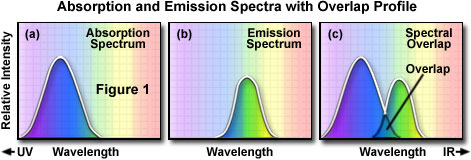
\includegraphics[scale=0.80]{img/CAP1stokes.jpg}
 \caption{ \small{Shift di Stokes.} In figura (a) si trova lo spettro di eccitazione incidente sul fluoroforo; in figura (b) lo spettro di emissione del fluoroforo; in figura (c) i due spettri sono mostrati sovraimposti, per evidenziare come vi sia una sovrapposizione fra i due.}
 \label{fig:stokes}
\end{figure}

Una volta che la molecola ha assorbito la radiazione incidente, si trova in uno degli stati vibrazionali di un livello energetico eccitato. 
Essendo soggetta a collisioni con le molecole circostanti, rilascia parte della sua energia sotto forma non radiativa, scendendo nella scala dei livelli vibrazionali interni allo stato eccitato. 
A questo punto, a seconda dell'intorno molecolare, la molecola può ritornare al suo stato fondamentale seguendo uno dei due seguenti processi:
\begin{description}
 \item [Processo non radiativo:]
Se le molecole circostanti sono in grado di assorbire la restante energia elettronica della molecola eccitata, quest'ultima completa il suo rilassamento in modo non radiativo, con conseguente liberazione di calore. 
Ciò permette alle molecole circostanti di attivare gradi di libertà vibrazionali, rotazionali e traslazionali, e perciò, come effetto complessivo, si ha un aumento dell'energia termica.
 \item [Processo radiativo:]
Se le molecole circostanti non sono in grado di assorbire la restante energia allora la molecola subisce un decadimento radiativo, ossia l'energia in eccesso viene liberata sotto forma di fotoni, aventi energia minore rispetto a quella dei fotoni che hanno causato l'eccitazione. 
Tale processo dà luogo ad un evento di emissione spontanea che può essere, a seconda dei casi, fluorescenza o fosforescenza.
\end{description}
La distinzione tra fluorescenza e fosforescenza fu originariamente fatta in base al tempo di vita della radiazione: nella fluorescenza la luminescenza cessa quasi subito dopo aver eliminato la radiazione eccitante, mentre nella fosforescenza la radiazione continua ad essere emessa, almeno per un breve lasso di tempo, anche dopo aver eliminato la sorgente eccitante. 
Infatti i materiali fluorescenti cessano di essere luminosi al cessare dello stimolo che ne determina la luminosità, mentre nei materiali fosforescenti la luce continua ad essere emessa per un certo periodo dopo la fine dello stimolo.

Con l'avanzare degli studi in tale ambito, si scoprì una più profonda distinzione tra i due fenomeni, legata alla natura degli stati elettronici coinvolti nelle transizioni responsabili dell'emissione di radiazione.
Quando un elettrone viene promosso da uno stato fondamentale, solitamente di singoletto, ($S_0$) ad uno eccitato, esso può mantenere lo spin originario oppure invertirlo: se l'eccitazione avviene con ritenzione dello spin si parla di stato di singoletto ($S_1$), se invece il passaggio allo stato attivato avviene con inversione dello spin si parla di stato di tripletto ($T_1$) (\figurename~\ref{fig:spin}). 
Allo stato di singoletto compete un'energia più alta e una vita media che va da $10^{-11}$ s a $10^{-9}$ s, mentre lo stato di tripletto ha energia inferiore e vita media che va da $10^{-3}$ s a $10^{1}$ s.

\begin{figure}
 \centering
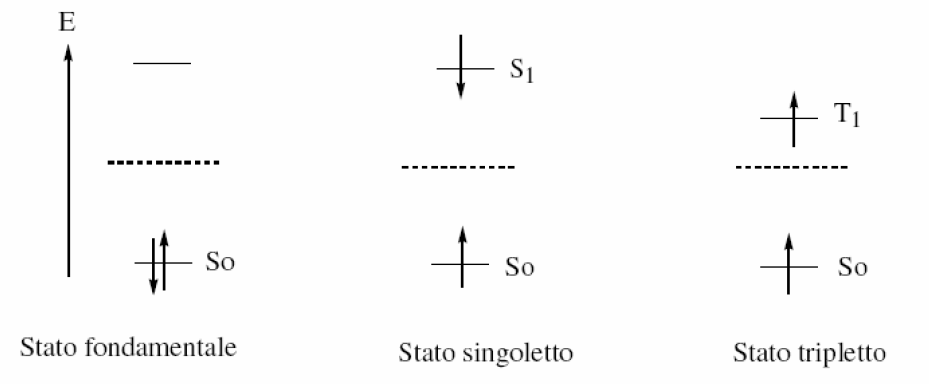
\includegraphics[scale=.40]{img/CAP1spin.png}
 \caption{\small{ Rappresentazione dei differenti stati elettronici. Lo stato fondamentale $S_0$ (sinistra), in seguito ad
eccitazione, può mutare nello stato di singoletto $S_1$ (centrale) o nello stato di tripletto $T_1$ (destra). }}
 \label{fig:spin}
\end{figure}

Per analizzare meglio i vari processi coinvolti nella diseccitazione bisogna fare riferimento al diagramma di Jablonski (\figurename~\ref{fig:jablonski}).
A seguito dell'assorbimento di luce (A), una molecola nello stato fondamentale ($S_0$) viene eccitata, per la conservazione dello spin, a uno dei suoi stati elettronici di singoletto ($S_1, S_2,\ldots$). 
L'energia vibrazionale della molecola eccitata viene trasferita a molecole vicine in seguito a collisioni e perciò vi è sempre un rapido ritorno al più basso livello vibrazionale dello stato di singoletto eccitato, senza emissione di radiazioni.
Questo fenomeno di rilassamento vibrazionale (R.V.) viene detto \textit{Conversione Interna} (C.I.) e si verifica in tempi dell'ordine di $10^{-12}$ s. 
C'è poi la possibilità che avvenga la \textit{Conversione di Sistema} (C.S.) o Intersystem Crossing, ossia che lo spin dell'elettrone, a causa degli urti con le altre molecole e dei moti molecolari, si inverta, comportando perciò il passaggio dallo stato di singoletto ($S_1$) allo stato di tripletto ($T_1$). 
La radiazione fluorescente (F) è generata da transizioni tra stati con la stessa molteplicità di spin (es. $S_1 \to S_0$). 
Nella fosforescenza (P), al contrario, la transizione coinvolta comporta sempre la variazione della molteplicità di spin (es. $T_1 \to S_0$).

\begin{figure}
 \centering
 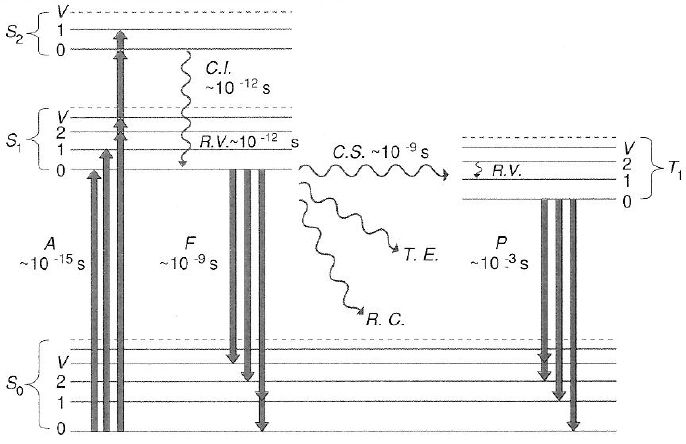
\includegraphics[scale=.45]{img/CAP1jablonski.JPG}
 \caption{\small{Diagramma di Jablonski. Nello schema $S_0$ indica il livello di energia elettronica fondamentale; $S_1$ ed $S_2$ sono rispettivamente il primo ed il secondo livello elettronico eccitato di singoletto; $T_1$ è il primo livello di tripletto. Sono indicati anche i sottolivelli di energia vibrazionale, in ordine di energia crescente, con $V_0, V_1, ...$, mentre non sono rappresentati i sottolivelli rotazionali.}}
 \label{fig:jablonski}
\end{figure}

I parametri tipici della fluorescenza sono:
\begin{description}
\item [Tempo di vita:]
Esso è definito come tempo medio di permanenza della molecola nello stato eccitato e per la fluorescenza è solitamente dell'ordine dei nanosecondi.
\item [Trasmittanza:]
Essa è definita, tramite la legge di Lambert-Beer, come rapporto tra l'intensità della luce trasmessa attraverso un mezzo di spessore s e l'intensità incidente: $$ T=\frac{I}{I_0} = e^ {k_\lambda s}$$ dove $k_\lambda$ è detto \textit{coefficiente di estinzione} ed è un parametro dipendente dal mezzo e dalla lunghezza d'onda della luce incidente.
\item [Efficienza quantica o resa:] 
Essa è definita come il rapporto tra il numero di fotoni emessi rispetto a quelli assorbiti. 
Questo coefficiente può assumere un valore compreso tra 0 (molecola non radiativa) e 1. I fluorofori hanno una resa quantica tipicamente non superiore a 0.1 per evitare fenomeni di re-emissione \cite{quantumyield}.
\end{description}


\subsection{Meccanismi di fading}

Esistono casi in cui la fluorescenza di una molecola può essere ridotta di intensità o addirittura annullata. 
Il termine che si usa per descrivere tale fenomeno è \textit{fading}, a sua volta distinguibile in quenching e photobleaching.
Entrambi i processi riducono il valore della resa quantica e il tempo di vita della fluorescenza.

\subsubsection*{Photobleaching}
Il meccanismo del photobleaching è dovuto a reazioni fotochimiche, provocate dalla luce di eccitazione, che variano in modo irreversibile la composizione del fluorocromo, rendendolo non più fluorescente. 

Tale fenomeno è oggi ancora poco conosciuto.
Esso coinvolge infatti molti fattori e può differire da un campione all'altro o anche da parti distinte di uno stesso.
L'assorbimento di luce comporta l'aumento del numero di molecole nello stato eccitato; essendo questo molto più reattivo di quello fondamentale, si ha che una piccola ma significativa frazione di molecole si trova coinvolta in nuove reazioni fotochimiche, a discapito dell'emissione di fluorescenza. 
Tali reazioni avvengono per lo più con ossigeno molecolare e causano la produzione di nuove molecole, che possono essere non-fluorescenti o addirittura incapaci di assorbire la luce incidente.
Ovviamente la quantità di photobleaching dipende dall'intensità della luce di eccitazione e risulta variabile durante il periodo di illuminazione: nei primi millisecondi di irraggiamento non è presente, successivamente aumenta in modo molto veloce per pochi secondi ed infine continua a procedere  più lentamente, andando ad attenuarsi.

Per ristabilire le proprietà fluorescenti del fluoroforo si può privare il campione della luce, mentre mantenuto a basse temperature. 
Inoltre, per evitare direttamente il fenomeno di photobleaching si può sfruttare un impulso di eccitazione molto breve o un fluorocromo particolarmente fotostabile.

Il fenomeno del photobleaching può essere anche indotto volontariamente per studiare il recupero di fluorescenza in un certo campione. 
Tale tecnica prende il nome di \textit{Fluorescence Recovery After Photobleaching} (FRAP) (\figurename~\ref{fig:FRAP}).

In particolari casi, sottoporre il campione alla luce di eccitazione per periodi prolungati può comportare un effetto totalmente opposto al photobleaching, detto \textit{photoactivation}. 
Difatti la manifestazione di tale fenomeno fa sì che la fluorescenza osservata, anzichè diminuire con il crescere del tempo di esposizione, aumenti rispetto al livello inizialmente mostrato. 
Nel caso in cui le cellule coinvolte siano cellule vitali, questo fenomeno può produrre effetti tossici molto dannosi.

\begin{figure}
 \centering
 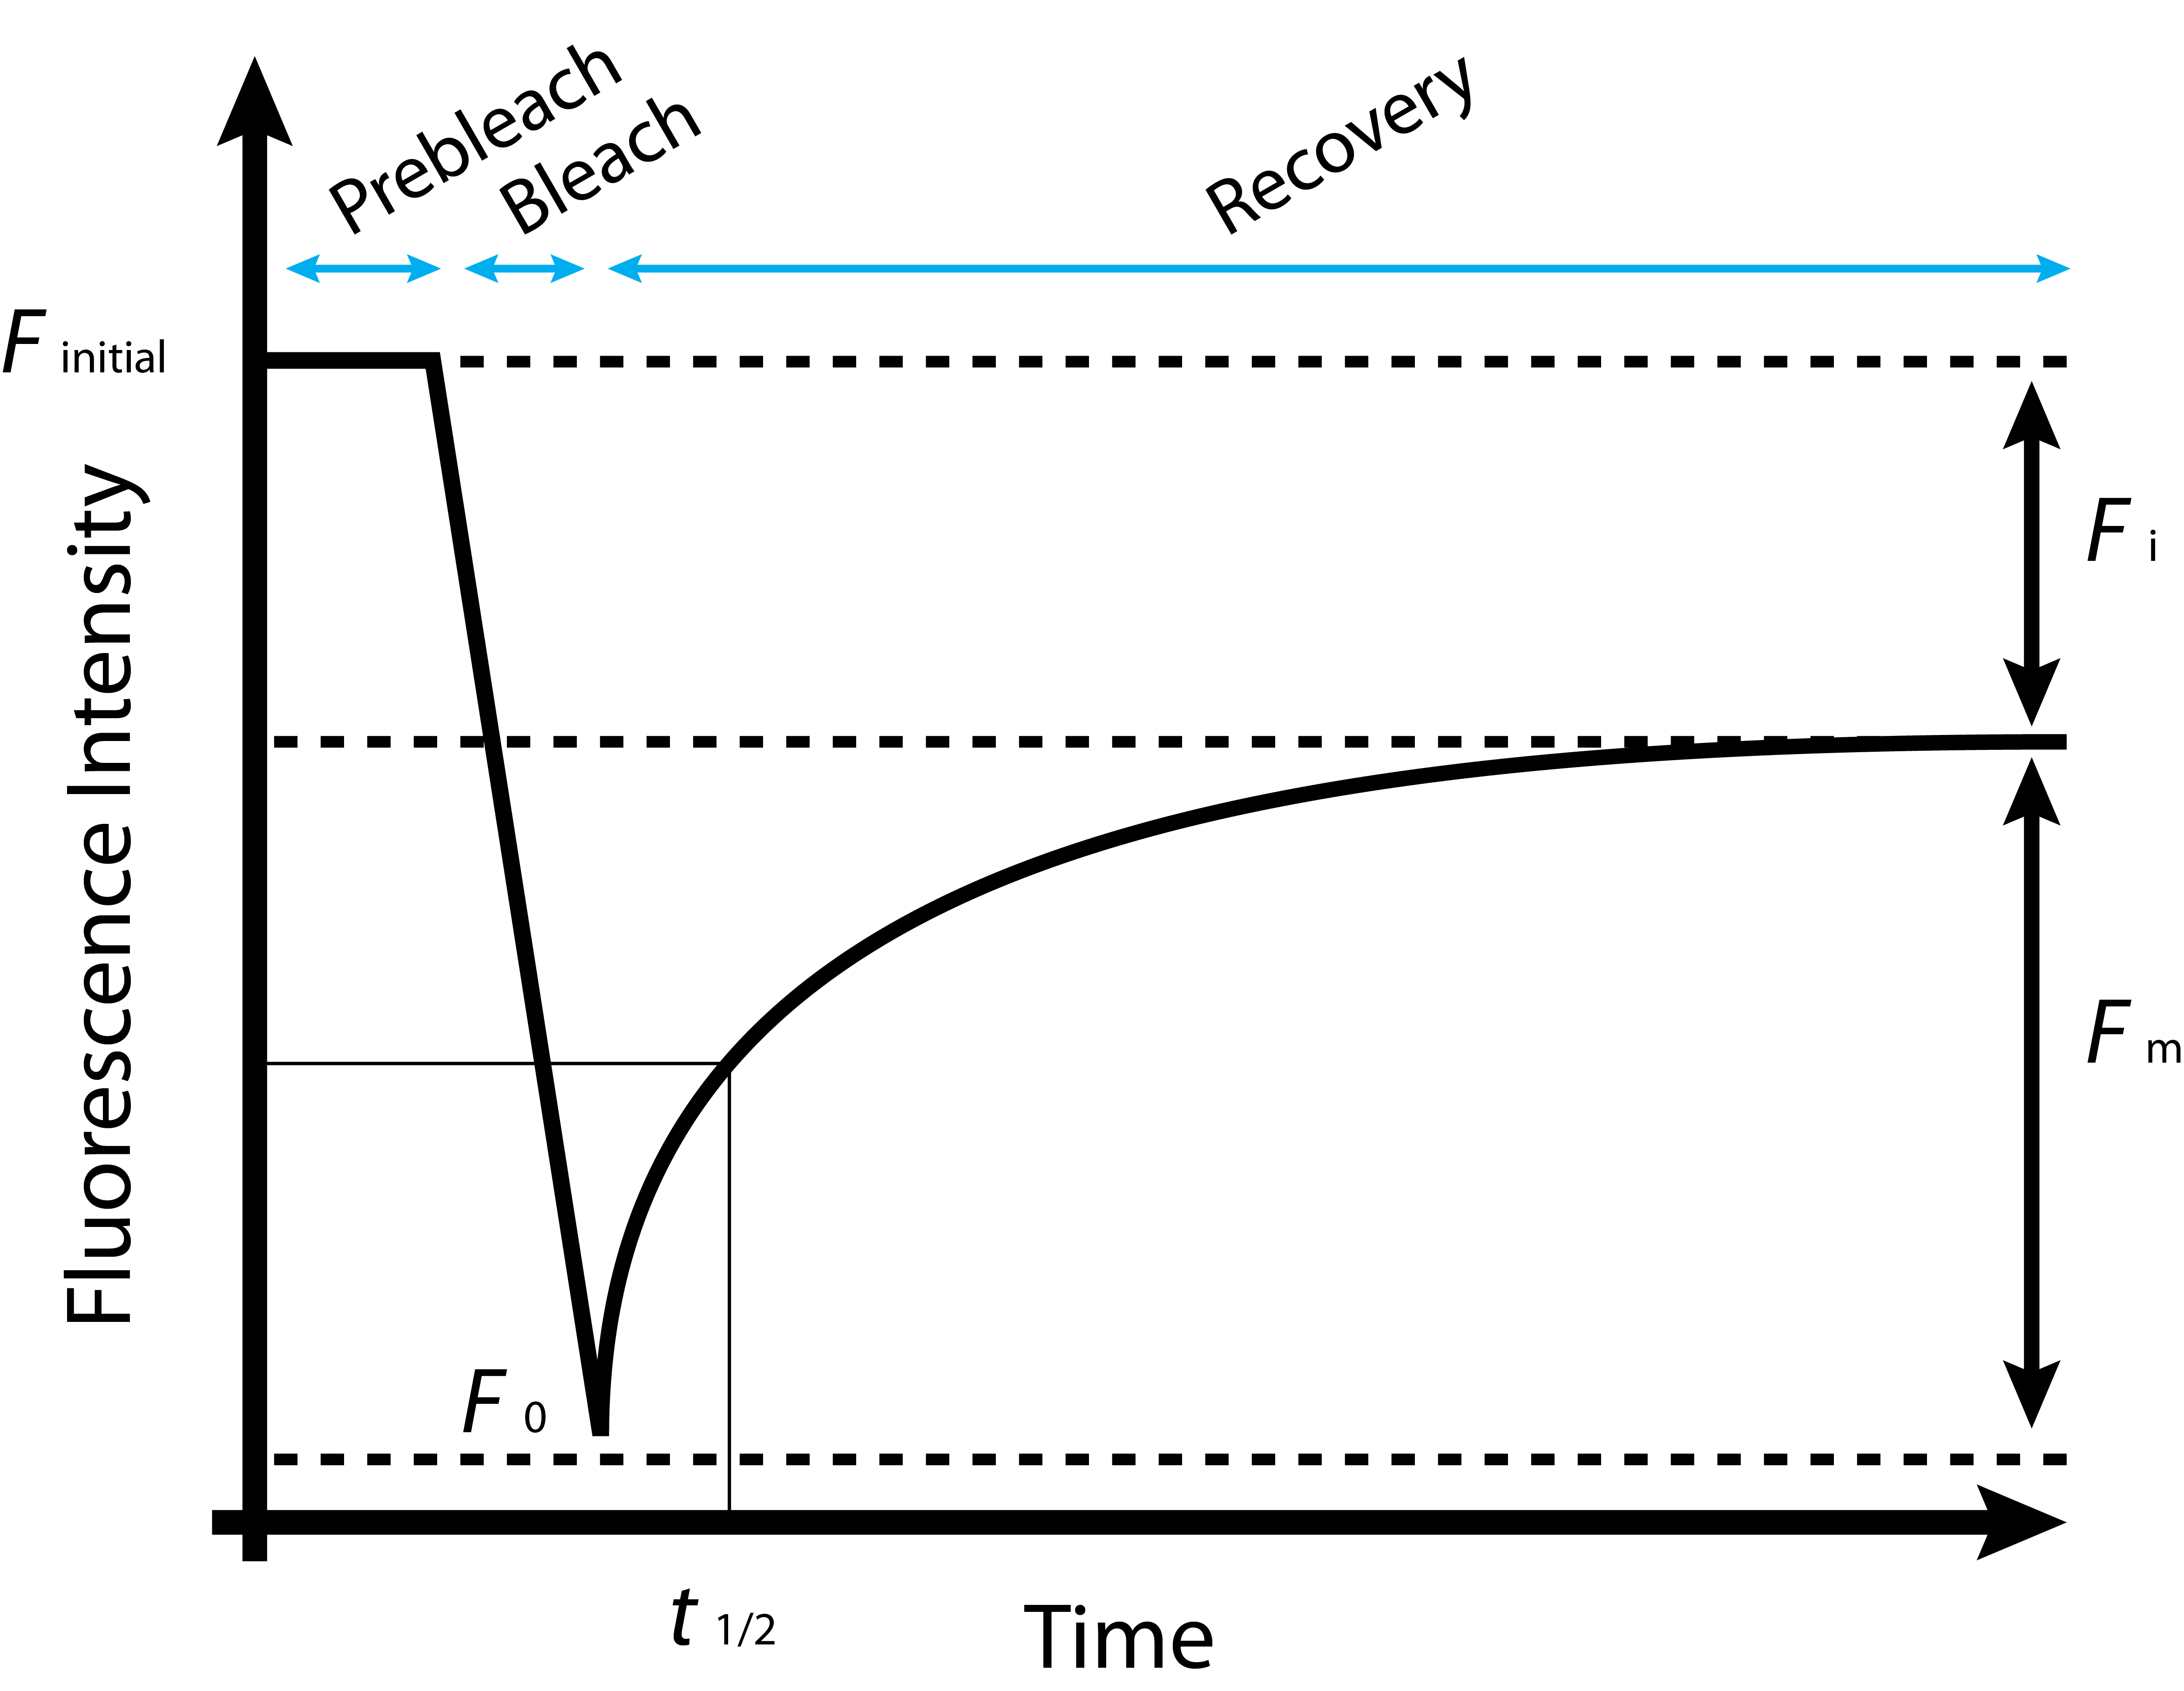
\includegraphics[scale=1]{img/CAP1FRAP.png}
 \caption{\small{Curva del FRAP. $F_{initial}$ ed $F_0$ sono rispettivamente l'intensità di fluorescenza antecedente ed immediatamente successiva al photobleaching; $F_m$ ed $F_i$ sono rispettivamente la frazione mobile ed immobile, ossia la frazione che contribuisce o no al recupero; $t_{1/2}$ è il tempo di recupero di metà frazione mobile.}}
 \label{fig:FRAP}
\end{figure}

\subsubsection*{Quenching}
Il meccanismo di quenching è dovuto alla presenza di molecole nel sistema, le quali comportano un processo di disattivazione in grado di ridurre la fluorescenza. Vengono solitamente distinti quattro tipi di quenching \cite{quenching}:
\begin{description}
\item [Quenching da temperatura:]
La fluorescenza decresce all'aumentare della temperatura dall'1\% al 5\%, a seconda del campione in esame. 
La causa è probabilmente da associare all'aumento di energia cinetica, quindi all'incremento delle collisioni molecolari, che provoca una maggior probabilità di transizione non radiativa verso lo stato fondamentale.

\item [Quenching da impurità o dinamico:]
La fluorescenza può diminuire o aumentare a causa della presenza di altre molecole nel mezzo.

Una molecola eccitata può trasferire il suo eccesso di energia ad una molecola adiacente che passa quindi nel suo stato eccitato, da cui potrà decadere
secondo ognuno dei meccanismi descritti precedentemente. 
Se l'accettore è non-fluorescente si avrà come risultato un fenomeno di quenching. 
Dato che il trasferimento di energia dal marcatore all'impurità può essere molto efficiente e può aver luogo fino a distanze di un micrometro, una concentrazione molto piccola di impurità può produrre un alto valore di quenching. 
Uno dei quenchers più noti è l'ossigeno molecolare che causa una grande riduzione nella fluorescenza, sino ad annullarla completamente. 
Ciò può essere evitato introducendo nel mezzo di coltura un agente riduttivo.
D'altra parte può anche accadere che l'accettore sia fluorescente ed in tal caso la luminescenza risulta incrementata dalla presenza dell'impurità.

Quest'ultimo tipo di quenching dinamico può essere sfruttato in modo positivo, per esempio nella cosiddetta \textit{F\"{o}rster Resonance Energy Transfer} (FRET o FET). 
Essa consiste nel trasferimento dell'eccitazione di una molecola donatrice ad una accettrice attraverso un processo non radiativo di interazione dipolo-dipolo.
La FRET ha varie caratteristiche: varia come $1/R^6$ e di conseguenza dipende strettamente dalla distanza donatore-accettore ($R$) che deve essere al più dell'ordine di $10\ nm$; necessita la sovrapposizione dello spettro di emissione del donatore con quello di eccitazione dell'accettore; dipende dall'orientazione relativa dei momenti di dipolo di transizione delle due molecole.
\item [Quenching statico:]
Esso si verifica quando le molecole del donatore e dell'accettore si trovano nello stato fondamentale, invece che in quello eccitato, e si legano insieme a formare un'unica molecola, anch'essa nello stato fondamentale ma non più fluorescente, avente un unico spettro di assorbimento. 
La causa è spesso legata ad effetti di idrofobia, ossia le due molecole si uniscono insieme per minimizzare il contatto con l'acqua.
\item [Quenching da concentrazione:]
Normalmente con l'aumentare della concentrazione del fluorocromo aumenta la quantità di fluorescenza. 
Tuttavia a concentrazioni molto elevate interviene il cosiddetto quenching da concentrazione, che comporta una riduzione della fluorescenza.
Questo può avvenire per aggregazione delle molecole del fluorocromo (come ad esempio nelle porfirine) oppure per trasferimento non radiativo di energia fra molecole identiche \cite{concquenc}.
\end{description} 


\section{Sonde fluorescenti}

Sia nel mondo vegetale che nel mondo animale, diverse sostanze naturali manifestano una fluorescenza intrinseca, detta anche \textit{autofluorescenza}.
Ne sono esempi le clorofille, molti pigmenti naturali (in particolare quelli di natura lipidica), alcuni amminoacidi (es. triptofano e tirosina), molti enzimi, coenzimi (es. NAD e NADH), cofattori (es. FAD e FADH) e molecole aromatiche. 
Tuttavia la maggior parte delle molecole biologiche di interesse biofisico non sono autofluorescenti all'interno degli intervalli spettrali sfruttati e anche quelle che lo sono, in genere, non possono essere distinte tra loro sulla base della loro fluorescenza intrinseca.

Per ovviare a ciò, Max Haitinger nel 1933 introdusse l'uso della fluorescenza secondaria nello studio dei preparati biologici, ossia aggirò tale problema utilizzando dei marcatori esterni, detti comunemente sonde o \textit{probes} fluorescenti. 
Da allora la procedura comunemente usata in microscopia è quella di marcare gli elementi che si vogliono studiare con fluorofori, che si legano a target specifici delle molecole di interesse, le quali, dopo opportuna eccitazione, potranno essere selettivamente rivelate grazie al segnale luminoso emesso dalle sonde. 

Ovviamente introdurre un agente esterno all'interno di un componente biologico non è così banale, infatti bisogna fare in modo che rispetti tutte le esigenze della cellula: il marcatore deve raggiungere il target e non allontanarsi da esso durante l'intera rilevazione; una volta \textit{in situ} il probe idealmente si deve comportare come un agente passivo che non induce perturbazioni significative nelle strutture o nelle funzioni biologiche che si vogliono studiare; infine si deve cercare di evitare che tramite il processo di misura si creino effetti negativi come fading e fototossicità.

I primi fluorofori usati erano semplici coloranti, perciò non specifici, e per questo si legavano a costrutti presenti praticamente ovunque nella cellula, producendo un segnale molto diffuso. 
Poi, con l'avanzare delle conoscenze biochimiche si trovarono sonde organiche, inorganiche o chimiche in grado di marcare costrutti molto specifici all'interno della cellula (es. nucleo, membrana, mitocondri, etc) e si introdussero protocolli sperimentali adeguati. 
La tecnologia attuale permette persino di sfruttare fluorocromi in grado di marcare solo particolari ioni, come ad esempio $Ca^{2+}$, $Mg^{2+}$, $Na^{2+}$, $Cl^-$ ed $O_2$.

Le proprietà che caratterizzano maggiormente i marcatori fluorescenti sono:
\begin{itemize}
\item Spettri di eccitazione ed emissione, importanti per la scelta del fluoroforo più adatto al proprio apparato sperimentale. 
Il primo si sceglie in modo da essere il più possibile centrato sulla lunghezza d'onda emessa dalla sorgente di luce, mentre il secondo deve poter essere rilevabile dagli strumenti a disposizione. 
\item Efficienza quantica, per avere il miglior segnale in fluorescenza rilevabile con i rivelatori utilizzati. 
\item Affinità con i diversi costrutti molecolari e tessuti subcellulari.
\item Modalità con cui possono penetrare all'interno della cellula.
\end{itemize}
Perciò, per la scelta del protocollo sperimentale atto alla marcatura, è fondamentale analizzare le specifiche dei vari coloranti, disponibili su database online. 
In \tablename~\ref{TABfluo} ne vengono riportati alcuni di uso comune.

\begin{table}[!ht]
 \begin{center}
\begin{small}
\begin{tabular}{lcc}
\hline\hline
\textbf{Colorante}&\textbf{Eccitazione}&\textbf{Emissione}\\
&\textbf{\small{(nm)}}&\textbf{\small{(nm)}}\\
\hline
\textbf{Fluorofori comunemente impiegati}&&\\
Fluoresceina-5-isotiocianato (FITC)&496&518\\
Isotiocianato di tetrametilrodamina (TRITC)&550&570\\
Tetrametilrodamina&554&576\\
Lissamina rodamina&572&590\\
Rosso Texas&592&610\\
\hline
\textbf{Coloranti per il nucleo}&&\\
4',6'-Diamidino-2-fenilindolo cloridrato (DAPI)&359&461\\
\hline
\textbf{Indicatori di calcio}&&\\
Indo-1&380&400/475\\
Fluo-2&340/380&510\\
Fluo-3&506&526\\
\hline
\textbf{Molecole reporter}&&\\
Proteina fluorescente verde (GFP)&395/475&509\\
DsRed&558&583\\
\hline
\textbf{Coloranti per i mitocondri}&&\\
Rodamina 123&507&529\\
\hline\hline
\end{tabular}
\caption{\small{Caratteristiche dei fluorofori di uso comune.}}
\label{TABfluo}
\end{small}
\end{center}
\end{table}


\subsection{Tecniche di marcatura}

Dall'analisi delle proprietà dei vari fluorocromi sono nate cinque principali tecniche specifiche di marcatura \cite{tecniche}:
\begin{enumerate}
\item tecnica di marcatura con coloranti fluorescenti;
\item tecnica di immunofluorescenza;
\item tecnica dell'ibridazione fluorescente in situ (FISH);
\item tecnica di marcatura con proteine fluorescenti;
\item Quantum Dots (QD).
\end{enumerate}

\subsubsection*{Marcatura con coloranti fluorescenti}
Nella tecnica di marcatura con coloranti fluorescenti le sonde sono assorbite direttamente dalla cellula, sfruttando solitamente i gradienti di concentrazione o il potenziale di membrana, ed in questo modo esse si concentrano in zone intracellulari specifiche.
Con tale metodo è possibile anche eseguire misure quantitative delle cellule vive che hanno assorbito il colorante fluorescente, dato che appaiono intensamente colorate su sfondo scuro. 

\subsubsection*{Immunofluorescenza}
La tecnica di immunofluorescenza si basa su anticorpi legati chimicamente a fluorofori, così da sfruttare successivamente il legame altamente specifico anticorpo-proteine. 
Dato che gli anticorpi sono molecole che si legano selettivamente a specifiche parti della cellula, in tal caso non sarà più il fluorocromo a decidere il legame, ma direttamente la molecola biologicamente attiva.

Questo metodo presenta come vantaggio il poter ottenere informazioni molto precise sia dal punto di vista spaziale che della specificità del legame, a discapito di dell'intensità, che risulta in tal caso debole a causa della piccola quantità di colorante legato.
Tuttavia il segnale può essere amplificato utilizzando la tecnica di \textit{immunofluorescenza indiretta}: un anticorpo specifico non marcato, detto anticorpo primario, diviene target di numerosi anticorpi secondari marcati da uno specifico fluoroforo. 
Solitamente per tale scopo si sfruttano come coloranti la fluoresceina, che emette nel verde se eccitata con luce blu, e la rodamina, che emette nel rosso se eccitata con luce giallo/verde.

\subsubsection*{Ibridazione fluorescente in situ}
La tecnica dell'ibridazione fluorescente in situ (FISH, \textit{Fluorescence In Situ Hybridization}) sfrutta probes che si legano in modo estremamente selettivo ad alcune regioni del cromosoma. 
Tale metodo permette di rilevare e localizzare la presenza/assenza di specifiche sequenze di DNA.

\subsubsection*{Marcatura con proteine fluorescenti}
La tecnica di marcatura con proteine fluorescenti sfrutta tecniche di ingegneria molecolare, in grado di modificare geneticamente una cellula eucariote rendendola capace di produrre una proteina fluorescente, ma senza alterarne la sua normale funzionalità. 
In questo modo la proteina marcata può essere sfruttata come tracciante (oltre che marcatore), ossia può essere seguita nel corso della sua sintesi, dalla compartimentazione intracellulare sino alle interazioni con le diverse strutture cellulari.

Il fatto che le proteine fluorescenti possano essere fuse alla proteina d'interesse così da rendere il targeting molto preciso è un grande pregio rispetto ai coloranti organici. 
I vantaggi di questo metodo biomolecolare sono soprattutto il non avere bisogno di tecniche invasive per visualizzare in cellule vive una proteina oggetto di studio, a differenza di quel che accade per esempio nella tecnica di immunofluorescenza dove le cellule devono essere precedentemente fissate; l'assenza di problemi di loading del fluoroforo, di rumore di fondo, di interazioni tra colorante ed ambiente circostante e tra le stesse molecole di fluoroforo ed infine l'alta precisione del targeting in quanto la proteina è prodotta dalla cellula stessa. 
Le difficoltà risiedono invece per lo più nell'ottimizzazione delle tecniche di trasfezione, attraverso cui la cellula viene geneticamente modificata, così da produrre la proteina di interesse.

Tra le più famose proteine fluorescenti vi sono la \textit{Green Fluorescent Protein} (GFP), isolata dalla medusa ``Aequorea Victoria'', e la \textit{Red Fluorescent Protein} (RFP), isolata dal corallo ``Discosoma'' (\figurename~\ref{fig:proteine}). 
La fluorescenza intrinseca di queste proteine è dovuta alla presenza di triptofano.

\begin{figure}
 \centering
 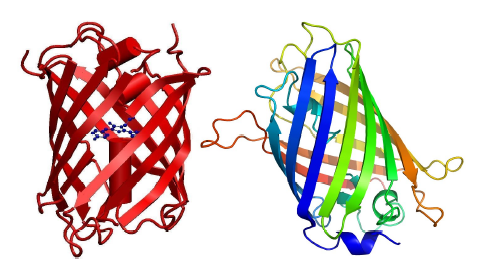
\includegraphics[scale=.50]{img/CAP1proteine.png}
 \caption{\small{ Struttura tridimensionale della RFP (sinistra) e della GFP (destra).}}
 \label{fig:proteine}
\end{figure}

\subsubsection*{Quantum Dots (QD)}
I Quantum Dots (QD) sono una classe di fluorocromi sviluppata negli ultimi anni sulla base di nuove competenze in ambito nanotecnologico.
Essi sono costituiti da un nucleo semiconduttore di cadmio-selenio ($ CdSe $) ricoperto da uno strato di solfato di zinco ($ ZnS $), necessario per migliorare l'efficienza quantica e la fotostabilità. 
Questi nanocristalli hanno dimensioni comparabili con le proteine (es. GFP) e, se eccitati ad opportune lunghezze d'onda, emettono fluorescenza, in colori differenti a seconda della dimensione della loro struttura (\figurename~\ref{fig:QD}).  
Infatti è il diametro del nucleo semiconduttore che determina lo spettro di emissione del QD: all'aumentare della dimensione si ha un aumento della lunghezza d'onda. 
Ciò è dovuto al fatto che QD più grandi presentano livelli di energia più vicini tra loro, così da poter assorbire anche i fotoni meno energetici ed emettere a grandi lunghezze d'onda. 

\begin{figure}
 \centering
 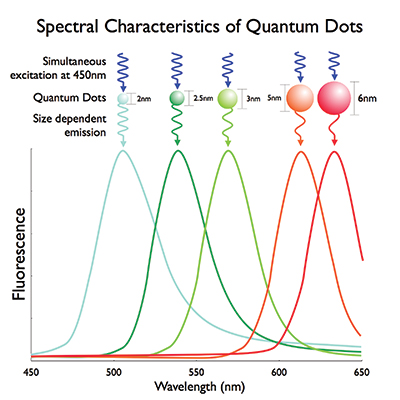
\includegraphics[scale=.60]{img/CAP1QD.jpg}
 \caption{\small{ Dimensione dei QD in relazione alla lunghezza d'onda di emissione.  I QD assorbono luce ad energia maggiore (lunghezza d'onda minore) e la convertono in luce ad energia minore (lunghezza d'onda maggiore). Monitorando la produzione dei Quantum Dots è possibile far sì che essi emettano luce ad ogni lunghezza d'onda dello spettro del visibile.}}
 \label{fig:QD}
\end{figure}

Un pregio di questa classe di fluorofori è legato agli spettri di eccitazione e di emissione: il primo risulta pressoché continuo e molto ampio, mentre il secondo è particolarmente piccato e simmetrico. 
In tal modo è possibile l'eccitazione di diverse specie di QD utilizzando un'unica fonte luminosa per la fluorescenza multipla, senza sovrapposizioni di segnale.
I QD emettono una fluorescenza circa 20 volte maggiore rispetto ai coloranti organici, la loro luminescenza ha lunga vita media ($30-100\ ns$) e presentano, grazie alla loro natura inorganica, l'ulteriore vantaggio di non subire photobleaching ossidativo, presente invece per i coloranti organici e le proteine fluorescenti. 
Tali proprietà diminuiscono le interferenze con l'autofluorescenza di background, rendendo i Quantum Dots molto utili nella monitorizzazione in continuo dei fenomeni biologici. 

Dato che le proprietà luminescenti dei QD ``nudi'' sono molto sensibili a vari tipi di interazione, si usa ricoprirli con materiali inorganici, solitamente solfato di zinco, che avendo un maggiore gap tra i livelli energetici migliorano le capacità luminescenti anche più del 50\% ($(CdSe)ZnS$ core-shell QDs).
Sotto questa forma però i QD non risultano biocompatibili e perciò è necessario sintetizzarli in presenza di composti idrofobici e inorganici, come l'ossido di trioctilfosfina (TOPO). 
In questo modo la loro superficie viene avvolta con una lunga catena alchilica, così da renderli solubili in solventi non polari, come il toluene. 

Una difficoltà riscontrabile con i QD è la loro traslocazione all'interno della cellula. 
Tuttavia questo problema è stato in parte risolto mediante l'utilizzo di proteine di trasporto, il cui compito naturale è appunto quello di trasportare altre proteine dall'esterno all'interno della cellula grazie alle loro forti cariche positive.

I QD sembrano dunque essere la futura tecnologia per lo studio di alcuni processi dinamici intracellulari, come per esempio il tracciamento delle proteine recettore e la loro distribuzione nello spazio e nel tempo.



\clearpage{\pagestyle{empty}\cleardoublepage}

\chapter{Microscopia a fluorescenza}

\begin{flushright}\begin{small}\textit{"Man is the interpreter of nature,\\ 
science the right interpretation."}\\
- William Whewell -\\
\end{small}\end{flushright}

Questo capitolo si propone di descrivere un tipico microscopio a fluorescenza, ponendo in particolare l'attenzione sul microscopio Nikon Eclipse-Ti, e inoltre di esaminare le principali imperfezioni e difetti presenti nelle immagini con esso acquisite.

\section {Il microscopio a fluorescenza}

Il microscopio a fluorescenza permette di studiare campioni organici o inorganici sfruttando i fenomeni di luminescenza descritti nel precedente capitolo, piuttosto che quelli di riflessione ed assorbimento della luce, basilari invece per i microscopi ottici tradizionali. 
In genere tale strumento è in grado di funzionare anche come microscopio ottico convenzionale, permettendo così il confronto tra le immagini acquisite nelle due diverse modalità.

Questo tipo di microscopia è caratterizzata dalla marcatura specifica del target in esame con una sonda fluorescente (capitolo 1.3.1) e da una struttura base dello strumento, costituita da: sorgente di luce, filtri, obiettivo e sistema di rivelazione. 
La descrizione che segue fa riferimento ad un microscopio a fluorescenza rovesciato (\figurename~\ref{fig:micro}), ove l'ottica è posizionata al di sotto del tavolino porta oggetti. 
Tale scelta è stata fatta per poter comprendere più facilmente il funzionamento del microscopio Nikon Eclipse-Ti che verrà analizzato successivamente.

\begin{figure}
 \centering
 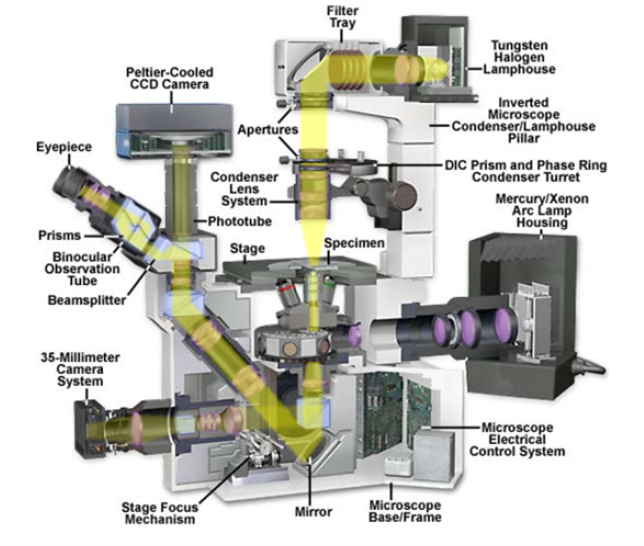
\includegraphics[scale=.60]{img/CAP2microrovesciato.jpg}
 \caption{\small{Schema ottico di un microscopio a fluorescenza rovesciato.}}
 \label{fig:micro}
\end{figure}

La sorgente di luce deve essere scelta in modo da massimizzare la quantità di fluoroforo eccitato, quindi l'intensità di emissione. 
Per questo motivo le lampade ad incandescenza non sono adatte, in quanto emettono prevalentemente luce di incandescenza nel rosso e nell'IR, con grande dispersione di calore. 
La scelta ricade in genere sulle \textbf{lampade a globo di quarzo} contenenti vapori di mercurio ad alta pressione, che soddisfano tutte le condizioni richieste. 

Esse vengono denominate con le sigle HBO 50 o HBO 100 a seconda della potenza dissipata e, a differenza delle lampade ad incandescenza, sfruttano il fenomeno delle scariche dei gas, caratteristica che gli conferisce uno spettro discreto. 
Questa lampada è costituita da un globo di quarzo, resistente alle alte pressioni, in cui sono fusi due elettrodi. 
Nella camera di combustione interna, contenente mercurio, viene generato e mantenuto attivo un arco voltaico tramite scariche ad alta tensione applicate agli elettrodi; il calore prodotto fa evaporare il mercurio, così da creare una situazione di sovrapressione. 

La lampada in esame emette luce molto intensa nello spettro UV, mentre nella parte del visibile l'intensità è più bassa, ma comunque sfruttabile per altre applicazioni. 
I picchi di intensità risultano proprio in corrispondenza dei cosiddetti ``picchi del mercurio'' (\figurename~\ref{fig:lamp}).

\begin{figure}
 \centering
 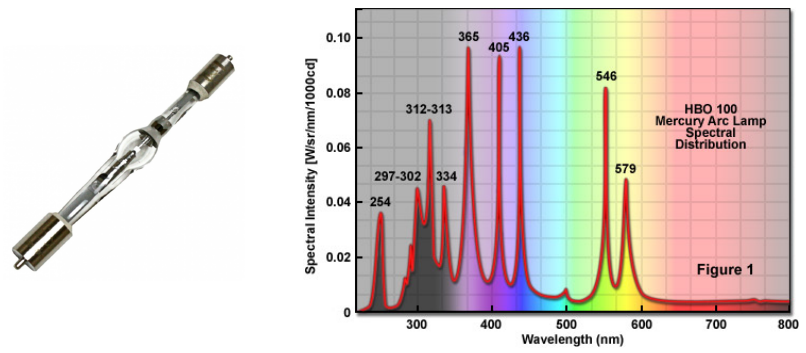
\includegraphics[scale=.48]{img/CAP2lampadaquarzo.png}
 \caption{\small{Arc-discharge fluorescence mercury lamp HBO 100 (sinistra) con associato spettro di emissione (destra).}}
 \label{fig:lamp}
\end{figure}

Come visto nel capitolo 1.3, il fascio di luce che raggiunge il campione deve avere una lunghezza d'onda prossima al picco di eccitazione del fluoroforo e inoltre il microscopio deve essere in grado di rivelare selettivamente la lunghezza d'onda di emissione di tale molecola, generando quindi un alto contrasto tra il background e le strutture fluorescenti.
Per soddisfare al meglio queste due richieste si sfruttano due filtri:
\begin{description}
\item[Filtro di eccitazione:]
Serve per filtrare la luce proveniente dalla sorgente prima che raggiunga il campione, lasciando passare così solo la lunghezza d'onda necessaria per l'eccitazione.
\item[Filtro barriera o di sbarramento:]
Serve per filtrare la luce proveniente dal campione, bloccando così la radiazione di illuminazione non assorbita dal fluoroforo e lasciando quindi passare solo quella di emissione. 
\end{description}
Per poter capire il loro utilizzo, servendoci della \figurename~\ref{fig:micro}, ripercorriamo il cammino ottico della luce di eccitazione: la luce emessa dalla lampada al mercurio passa attraverso l'illuminatore lungo un asse perpendicolare all'asse ottico primario del microscopio, attraversando una lente collettrice e un diaframma di apertura e centratura variabile. 
La luce viene poi filtrata dal filtro di eccitazione e incontra successivamente uno \textbf{specchio dicroico} (chromatic beamsplitter). 
Quest'ultimo è un filtro interferenziale specializzato nel riflettere le piccole lunghezze d'onda e trasmettere quelle più alte; esso è posto su in piano inclinato a 45° rispetto alla direzione della luce incidente e riflette la luce a 90° rispetto alla stessa direzione, proiettandola attraverso l'obiettivo, sino a colpire il campione. 
Il segnale di fluorescenza emesso dal campione viene quindi raccolto dal medesimo obiettivo e passa attraverso lo specchio dicroico, in virtù del fatto che la sua lunghezza d'onda risulta maggiore di quella di eccitazione, per lo shift di Stokes. 
Questo segnale di emissione passa attraverso il filtro di sbarramento e infine raggiunge i dispositivi per la formazione dell'immagine.

Spesso i filtri e lo specchio dicroico vengono montati in un unico blocco ottico detto \textit{filter cube} (\figurename~\ref{fig:cube}). 
Notiamo quindi che è proprio in base a tali elementi che si stabilisce quali molecole fluorescenti usare, infatti è possibile sfruttare unicamente quei fluorofori con lunghezze di eccitazione e di emissione corrispondenti a quelle trasmesse dai filtri. 
Inoltre, combinando vari filtri è possibile l'osservazione di un gran numero di fluorocromi con differenti proprietà di eccitazione ed emissive.

\begin{figure}
 \centering
 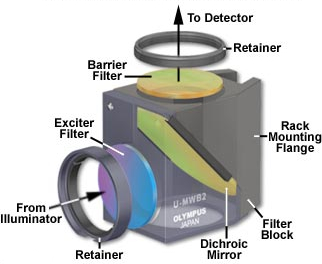
\includegraphics[scale=.65]{img/CAP2cube.jpg}
 \caption{\small{Schema ottico di un filter cube per microscopi a fluorescenza rovesciati.}}
 \label{fig:cube}
\end{figure}

Altro elemento fondamentale è certamente l'\textbf{obiettivo} e, come accennato, le sue lenti svolgono una duplice funzione: focalizzazione della luce di eccitazione sul campione (ancor più rispetto al sistema di lenti del condensatore presente in un microscopio convenzionale) e raccolta della luce di fluorescenza emessa. 

Gli obiettivi possono essere di diverso tipo e sono caratterizzati dalle informazioni riportate su di essi, come per esempio: fabbricante, ingrandimento ($4x,\ 10x,\ 20x,\ 40x,\ 60x\ o\ 100x$), requisiti per l'immersione ad aria, olio o acqua (in genere obiettivi con ingrandimento minore di $40x$ sono ad aria e quelli con ingrandimento pari o superiore a $40x$ sono ad immersione) e spessore del vetrino coprioggetti (solitamente $0.17\ mm$).  
Possono essere riportate anche informazioni relative alle correzioni per artefatti ottici, come aberrazioni cromatiche e appiattimento di campo.
Ne sono degli esempi le scritte ``fluo'' per lenti meno corrette o ``plan'' e ``plan apo'' per lenti con correzioni più fini. 

Altro parametro sempre presente sull'obiettivo è l'apertura numerica ($NA$, Numerical Aperture). 
Essa è una misura della capacità di una lente di raccogliere la luce del campione ed è definita dalla relazione:
$$ NA = n \cdot sin \theta $$
dove $n$ è l'indice di rifrazione del mezzo presente tra lente e campione e $\theta$ è l'apertura angolare della lente, ossia il semiangolo del cono di luce che entra nell'ottica. 
Il range di variabilità della $NA$ è solitamente tra 0.25, per obiettivi a basso ingrandimento e a secco (es. $10x$), e 1.45, per obiettivi ad immersione (es. da $40x$ a $100x$). 
In microscopia a fluorescenza è necessario utilizzare obiettivi con alta apertura numerica, così da massimizzare la quantità di luce raccolta dal campione \cite{NA}.
Infatti, la luminosità L dell'immagine, definita come flusso di fotoni per unità di superficie e di tempo ($W/m^2$), è legata all'apertura numerica tramite la relazione:
$$L  \propto  \frac {NA^4}{I^2}$$
dove $I$ è l'ingrandimento. 
Risulta quindi evidente che le immagini a fluorescenza più brillanti saranno raccolte da obiettivi con grande $NA$ e piccolo $I$; dei buoni valori sono per esempio $NA=0.75$ e $I=20x$.
D'altra parte il guadagno ottenuto aumentando l'apertura numerica, molto utile dato che le emissioni in fluorescenza risultano decisamente poco intense, comporta alcuni effetti indesiderati, come l'aumento dell'autofluorescenza e delle riflessioni da parte delle superfici delle lenti interne che riducono l'intensità finale. 
Tale problema può essere in parte marginato usando un liquido d'immersione, specialmente olio, così da eliminare la perdita di luce
causata dai riflessi sulle superfici e rendere l'immagine più chiara. 
Inoltre, una maggior apertura numerica migliora anche la risoluzione $d$ dell'immagine, poiché data dall'equazione:
$$d = 0.61 \ \frac {\lambda}{NA} $$
dove $\lambda$ è la lunghezza d'onda della luce di eccitazione.

Come visto precedentemente, nei microscopi a fluorescenza l'illuminazione è pensata in modo tale che sia la luce di eccitazione che quella di emissione passino per lo stesso obiettivo: ciò comporta numerosi vantaggi. 
Innanzitutto il fatto che l'obiettivo funzioni sia da condensatore che da dispositivo di formazione dell'immagine fa sì che l'allineamento condensatore-obiettivo sia sempre perfetto, che l'area illuminata dalla luce di eccitazione sia ristretta a quella che si osserva attraverso l'obiettivo e che sia disponibile tutta l'apertura numerica dell'obiettivo stesso; infine questa configurazione permette di combinare la tecnica della fluorescenza con alcune tecniche in luce trasmessa.


\subsection{Microscopio Nikon Eclipse-Ti}

Il microscopio a fluorescenza rovesciato Nikon Eclipse-Ti è stato acquistato alcuni anni fa dal Dipartimento di Fisica di Bologna per lo studio biofisico di alcuni effetti prodotti da radiazioni ionizzanti su cellule di fibroblasti umani, nell'ambito della ricerca sperimentale sull'invecchiamento fisiologico ed indotto dall'esposizione a radiazioni ionizzanti a differenti dosi. 

Tale microscopio può essere utilizzato sia per la microscopia in fluorescenza, sia per quella in campo chiaro a luce trasmessa.
Per poter rivelare la luce emessa dal campione è possibile sfruttare sia l'oculare che un sistema di rivelazione digitale, come per esempio una telecamera.
Nel caso in cui si utilizzi quest'ultimo sistema di rivelazione, le immagini verranno visualizzate sul monitor di un computer e registrate in formato digitale grazie ad appositi softwares, tramite cui è anche possibile elaborare ed analizzare le acquisizioni. 
La scelta di registrare le immagini rende inoltre possibile confrontare situazioni a tempi diversi e quindi creare una misura in dinamica, cosiddetta ``time-lapse''. 
La caratteristica principale di tale strumento è la possibilità di fare acquisizioni in vivo in time-lapse, anche per decine di ore, grazie ad un innovativo sistema di incubazione, in grado di mantenere in vita le cellule, integrato con il tavolino portaoggetti motorizzato ed un sistema di ``perfect focus''.

\begin{figure}
 \centering
 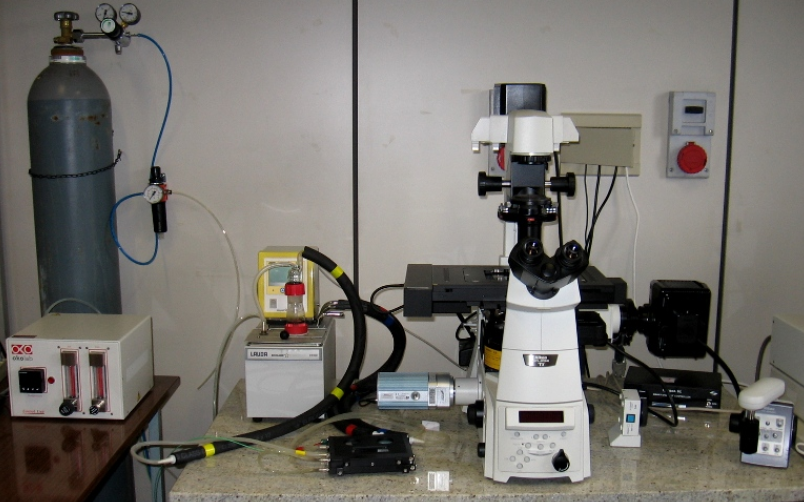
\includegraphics[scale=.45]{img/CAP2microNIKON.png}
 \caption{\small{Microscopio Nikon Eclipse-Ti.}}
 \label{fig:NIKON}
\end{figure}

Qui di seguito viene riportata una descrizione dei vari elementi che compongono il microscopio Nikon Eclipse-Ti (\figurename~\ref{fig:NIKON}):

\begin{description}

\item[Lampada diascopica:]
\'E una lampada alogena (TI-DH Dia Pillar Illuminator 12V/100W) per osservazioni in campo chiaro e contrasto di fase.

\item[Lampada episcopica:]
Si tratta di una lampada per la fluorescenza al mercurio HBO (arc-discharge fluorescence mercury lamp HBO) analoga a quelle descritte in precedenza.

\item[Obiettivi:]
Gli obiettivi disponibili sono $10x$, $20x\ Fluo$, $40x\ Super\ Fluo$, $60x\ Oil\ Fluo$ e rispettano, seppur con qualche compromesso, le esigenze sia dell'imaging cellulare in dinamica che dell'imaging in fluorescenza. 
Scegliere il giusto obiettivo è molto importante ai fini di un maggior segnale dal campione ed un miglior trasferimento di esso al sistema di rivelazione.

\item[Smart Shutter ultraveloce LAMBDA SC:]
Esso permette di decidere quando lasciare che la luce illumini il campione e quando no, senza dover spegnere manualmente la lampada sorgente.
Tramite software si può inoltre programmare ogni quanto aprire e chiudere lo shutter.

\item[Filter Cube:]
Questo microscopio è dotato di un meccanismo scorrevole che può contenere fino a sei cubi, così da disporre velocemente di sei combinazioni di filtri diversi \cite{Nikon1}. 
Attualmente dispone di 3 cubi, che permettono combinazioni di filtri per l'osservazione di fluorofori che emettono nel blu, nel rosso e nel verde, con eccitazioni tipiche dei coloranti più diffusi, che sono rispettivamente: DAPI, TRITC e FITC. 
I filtri sono denominati in associazione a tali fluorocromi, tuttavia presentano configurazioni di eccitazione e di emissione molto versatili, in quanto esiste un grande numero di fluorofori con proprietà compatibili con esse. 
In \tablename~\ref{TAB} sono riportate le bande di eccitazione e di emissione dei cubi a disposizione:

\begin{table}[!ht]
 \begin{center}
\begin{small}
\begin{tabular}{lccc}
\hline\hline
&\textbf{$\lambda$ eccitazione (nm)}&\textbf{$\lambda$ emissione (nm)}&\textbf{$\lambda$ dicroico (nm)}\\
\hline
\textbf{DAPI}&330 - 380&$\geq$ 420&400\\
\textbf{TRITC}&515 - 565&550 - 660&565\\
\textbf{FITC}&465 - 495&515 - 555&505\\
\hline\hline
\end{tabular}
\caption{\small{Bande dei tre filter cubes del Nikon Eclipse-Ti del Dipartimento di Fisica di Bologna.}}
\label{TAB}
\end{small}
\end{center}
\end{table}

\item[Telecamera:]

\begin{figure}
 \centering
 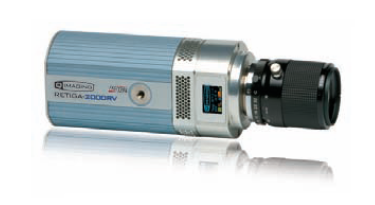
\includegraphics[scale=.60]{img/CAP2CCD.png}
 \caption{\small{Telecamera Qimaging, modello RETIGA-2000-RV.}}
 \label{fig:CCD}
\end{figure}

Il rivelatore CCD di cui è dotato il microscopio è una telecamera Qimaging, modello RETIGA-2000-RV (\figurename~\ref{fig:CCD}), in grado di rilevare segnali di bassa intensità, con un alto range dinamico e applicazioni rapide, caratteristiche che la rendono particolarmente adatta per l'imaging dinamico in vivo e in fluorescenza.
La telecamera presenta un sistema di raffreddamento che permette di regolare la temperatura fino a 30°C sotto zero, così da ridurre drasticamente il rumore termico, che costituisce un grande problema in quanto riduce il rapporto segnale-rumore nell'imaging dinamico.
Essa è sincronizzata con le lampade di illuminazione del microscopio, con il tavolino motorizzato, con il filter cube e lo shutter. 
Il rivelatore CCD ha 1.92 megapixel e produce un output a 12 bit in livelli di grigio.
È dotata di un filtro IR (infrarosso), posto di fronte al rivelatore, necessario per abbattere la componente IR che potrebbe provenire dal sistema di rilevamento del fuoco (Perfect Focus System). 
Infine, il tempo di esposizione può variare entro il range $10\ \mu s - 17.9\ min $, regolabile attraverso software.

\item[Sistema di incubazione:]
Il microscopio Nikon Eclipse-Ti è dotato di un supporto per il tavolino portaoggetti, adatto all'inserimento di un piccolo incubatore fabbricato dalla ditta Oko-Lab (\figurename~\ref{fig:okolab} e \figurename~\ref{fig:controllo}).
Al suo interno si crea un ambiente adatto alla sopravvivenza delle cellule, con una temperatura controllata, una miscela di aria e anidride carbonica fornita tramite bombola ed un certo tasso di umidità gestito da un apposito bagno termostatato.

\begin{figure}
 \centering
 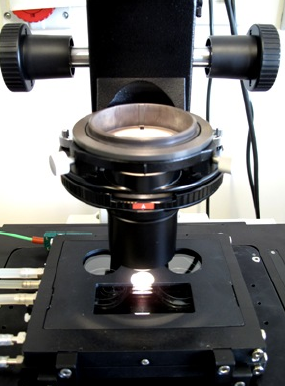
\includegraphics[scale=.60]{img/CAP2okolab.png}
 \caption{\small{Incubatore della Oko-Lab integrato con il tavolino portaoggetti del microscopio Nikon Eclipse-Ti.}}
 \label{fig:okolab}
\end{figure}

\begin{figure}
 \centering
 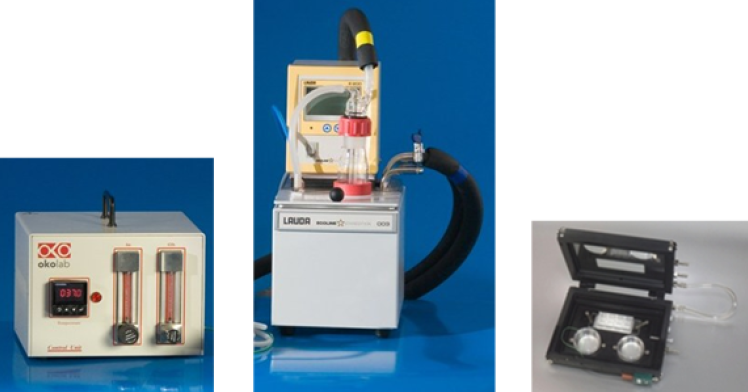
\includegraphics[scale=.45]{img/CAP2controllo.png}
 \caption{\small{Sistemi di controllo dell'aria e della $CO_2$ (sinistra), termostato a bagno termico (centrale) ed incubatore della Okolab (destra).}}
 \label{fig:controllo}
\end{figure}

Per creare e mantenere questo microclima all'interno dell'incubatore sono necessari diversi sistemi di controllo (\figurename~\ref{fig:controllo}). 
La temperatura è regolata attraverso un apposito software che la rileva costantemente sfruttando una termocoppia collegata all'unità di controllo. 
Essa è mantenuta costante grazie ad un termostato a bagno termico che tramite una resistenza scalda l'acqua, la inietta in un'intercapedine e, scorrendo lungo i bordi del piccolo incubatore, scalda l'aria al suo interno.
La stessa unità di controllo che regola la temperatura, se collegata ad una pompa ad aria compressa e ad una bombola di $CO_2$, permette all'operatore di regolare il flusso di aria ed anidride carbonica, creando in tal modo l'``atmosfera'' ideale per la vitalità delle cellule.
Infine, per quanto riguarda l'umidità è presente un'unità apposita, immersa nel bagno termico, in grado di produrre del vapore, successivamente immesso all'interno dell'incubatore.

\item[Perfect Focus System (PFS):]
Il PFS è un meccanismo hardware ideato dalla Nikon per poter contrastare gli spostamenti assiali del tavolino motorizzato ed evitare in tal modo la perdita del fuoco (vedere la sezione \ref{PFS}).

\item[Software Nis-Element 3.1:]
Esso è il software attraverso cui si gestiscono le varie funzionalità del microscopio, dalla creazione di sequenze di acquisizione spazio-temporali sino all'analisi delle immagini ottenute (vedere la sezione \ref{NisElements}).

\end{description}


\subsection{Perfect Focus System (PFS)}\label{PFS}

Supponendo che tutte le condizioni ambientali esterne al campione siano ideali, l'unico disturbo alla misura è la perdita intrinseca del fuoco dovuta ai gradienti termici, vibrazioni, instabilità meccaniche e un certo numero di altri fattori difficilmente eliminabili.

La Nikon ha affrontato questo problema progettando una soluzione hardware, detta \textit{Perfect Focus System} (PFS), pensata per contrastare gli spostamenti assiali in tempo reale nell'arco dell'intera acquisizione \cite{Nikon2}. 
Tale soluzione risulta molto utile specialmente negli esperimenti in cui si osservano più parti del campione, ove gli spostamenti macroscopici del tavolino motorizzato sono inevitabili.

\begin{figure}
 \centering
 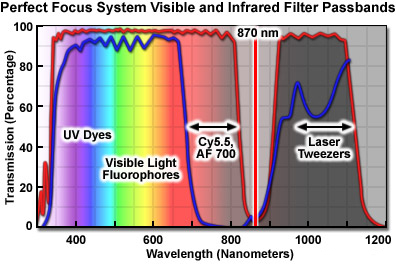
\includegraphics[scale=.70]{img/CAP2bande.png}
 \caption{\small{Bande di emissione dei marcatori fluorescenti e del LED a 870 nm.}}
 \label{fig:bande}
\end{figure}

Punto critico del PFS è il rilevamento accurato di un certo piano assiale che possa essere utilizzato come riferimento per stabilire con precisione la distanza che deve intercorrere tra la superficie della lente obiettivo ed il piano focale di interesse nel campione. 
A questo scopo il PFS utilizza un LED infrarosso a $870\ nm$ che non interferisce con i segnali raccolti dall'ottica dell'obiettivo: nè con la luce di eccitazione, né con quella emessa dai fluorofori, poiché presentano lunghezze d'onda di emissione comprese entro il range $[340\ -\ 770]\ nm$ (\figurename~\ref{fig:bande}).

Tale sistema di controllo del fuoco presenta come vantaggio la grande velocità di feedback, in quanto viene fornito dal PFS ogni $5\ ms$ (per altri meccanismi esistenti di mantenimento del fuoco viene fornito al più ogni $500\ ms$) e la distanza tra l'obiettivo e il campione viene mantenuta costante con una precisione assiale di $0.025\ nm$. 
Tuttavia il PFS presenta alcuni limiti di utilizzo, legati al tipo di campione e di supporto usati. 
Per esempio, nel caso di campioni immersi in mezzi acquosi occorre che lo spessore del mezzo sia di almeno $3\ mm$; la camera su cui sono coltivati i campioni deve avere un fondo di spessore compreso tra $150\ nm$ e $180\ nm$ per permettere una riflessione ottimale del segnale infrarosso; campioni troppo spessi o seminati su petri o vetrini di materiali diversi dal vetro, come per esempio la plastica, che presentano un forte scattering dell'infrarosso, non sono adatti per l'utilizzo del PFS. 

Infine bisogna osservare che l''unità PFS Nikon è situata nel gruppo ottico di sei obiettivi, situato tra la torretta dei filtri per la fluorescenza e il tavolino del microscopio; che i suoi controlli elettronici sono anch'essi all'interno del gruppo ottico e sono autosufficienti, cioè non richiedono un software supplementare per la loro gestione e che il PFS può essere attivato o disattivato tramite una leva che inserisce o meno lo specchio dicroico nel percorso ottico primario del microscopio.


\subsection{Software Nis-Element 3.1}\label{NisElements}

Nis-Element 3.1 è, come accennato, il software associato al microscopio Nikon Eclipse-Ti.
Tramite tale software le immagini possono essere osservate o in modalità ``live'', ovvero in tempo reale, oppure in modalità di ``visualizzazione'', cioè mostrando le immagini acquisite e salvate in precedenza, su cui è possibile avviare un'eventuale elaborazione attraverso gli strumenti di analisi delle immagini digitali di cui il programma dispone.

\begin{figure}
 \centering
 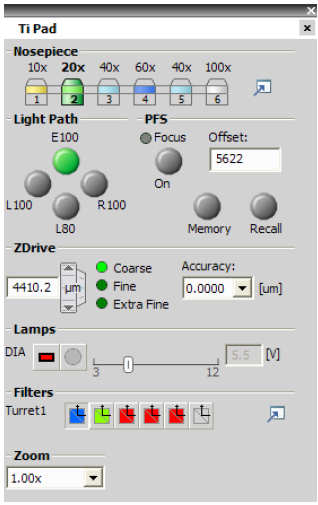
\includegraphics[scale=.50]{img/CAP2pannello.png}
 \caption{\small{Microscope Control Pad (Tipad).}}
 \label{fig:pannello}
\end{figure}

Nella schermata iniziale è presente un riquadro che visualizza l'immagine in esame ed il pannello ``Microscope Control Pad'', detto anche TiPad (\figurename~\ref{fig:pannello}), da cui l'utente può gestire i diversi componenti del microscopio. 
Tale pannello dispone delle seguenti sezioni di controllo:

\begin{description}
\item[Nosepiece:]
Permette la selezione dell'obiettivo da utilizzare durante l'osservazione e crea differenti configurazioni ottiche a seconda dell'obiettivo montato dall'utente sul corpo ottico del microscopio.

\item[Light Path:]
Questa box riproduce la stessa pulsantiera a croce presente alla base del microscopio (\figurename~\ref{fig:NIKON}), attraverso cui si seleziona il percorso ottico della luce. 
Le due modalità ``L100'' e ``R100'' mandano il 100\% del segnale rispettivamente all'uscita di sinistra e di destra, dove sono presenti i collegamenti per i rivelatori CCD; la modalità ``Eye'' direziona tutto il segnale verso l'oculare; la modalità ``L80'' direziona l'80\% del segnale verso l'uscita del rivelatore di sinistra ed il 20\% verso l'oculare.

\item[PFS:]
\'E il pulsante per l'attivazione e la disattivazione del Perfect Focus System. 
Quando la spia è verde significa che il PFS è attivato ed il fuoco non è più regolabile con la manopola tradizionale ma con quella del PFS. 
Una volta messa a fuoco l'immagine, cliccando sul pulsante Memory si può memorizzare l'offset della posizione scelta.

\item[Z Drive:]
Permette di decidere la sensibilità degli spostamenti assiali del tavolino motorizzato per la ricerca del piano focale nella modalità senza PFS inserito.
\'E possibile impostare tre differenti sensibilità: Coarse (grezzo), Fine (fine) e ExFine (extra fine).

\item[Lamp:]
Questa box permette l'accensione e la regolazione della potenza della luce di illuminazione per le osservazioni in luce trasmessa.

\item[Filters:]
Questa box permette di inserire nel percorso ottico primario del microscopio i diversi filter cubes necessari per la fluorescenza.
L'operatore può creare configurazioni differenti a seconda delle combinazioni di filtri di cui dispone, memorizzando per ciascuna le bande di lunghezze d'onda del filtro di eccitazione, di emissione e dello specchio dicroico.
Una volta impostati questi parametri il programma assocerà all'immagine monocromatica acquisita dalla telecamera, in una data combinazione di filtri, un colore fittizio corrispondente alla banda di lunghezza d'onda impostata per il filtro di emissione.
\end{description}

Ovviamente tale pannello non è l'unico presente, infatti si possono visualizzare altre interfacce: quella per la regolazione del tempo di esposizione e del guadagno del pixel della telecamera durante l'acquisizione o quella per la visualizzazione dell'istogramma dell'immagine acquisita.
Il software prevede anche la possibilità di salvare alcune configurazioni di utilizzo del microscopio, quindi memorizzare tutti i parametri del TiPad e le impostazioni di acquisizione della telecamera, ed attivarle ogni volta che viene premuto il pulsante associato alla configurazione desiderata. 

Nis-Element 3.1 permette inoltre di programmare vari tipi di acquisizione. 
In particolare, grazie al menu ``ND Acquisition'' (\figurename~\ref{fig:6D}), è possibile effettuare l'\textit{acquisizione in 6D}, ossia combinare a seconda delle esigenze dell'utente sequenze spaziali, temporali e vari tipi di filtri. 

\begin{figure}
 \centering
 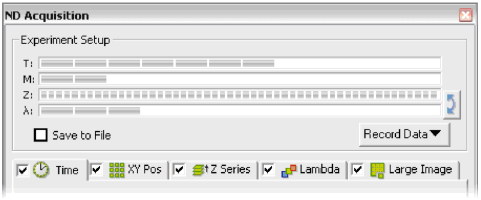
\includegraphics[scale=.70]{img/CAP26D.png}
 \caption{\small{Menu ND Acquisition per l'acquisizione in 6D.}}
 \label{fig:6D}
\end{figure}

Nel menu a tendina ``Time'' si impostano i parametri per l'\textit{acquisizione in time-lapse}, dove è possibile creare filmati in formato AVI. 
Via software si può impostare ogni quanto acquisire le immagini, da qualche $ms$ a qualche ora, tenendo presente che non è possibile acquisire le immagini ad intervalli temporali minori del tempo di esposizione settato per la telecamera. 
Le immagini vengono salvate in un file unico da cui è possibile estrarre solo alcuni fotogrammi o selezionare solo alcuni intervalli di tempo per produrre successivamente dei filmati separati, sempre in formato AVI. 
È inoltre possibile impostare diverse fasi di lavoro, salvate in file separati, e decidere per ciascuna fase il rate temporale di acquisizione e la durata totale dell'osservazione. 
La tendina ``XY Pos'' permette invece di impostare l'\textit{acquisizione in multi-point}, in cui si possono memorizzare varie posizioni (x, y, z), così da poter osservare più di un campo di vista all'interno del campione. 
Nel menu a tendina ``Z Series'' si imposta l'\textit{acquisizione in z-serie} che permette di acquisire immagini a diversi piani di fuoco e di visualizzarle poi in modalità tridimensionale, sfruttando un apposito algoritmo di deconvoluzione che elimina in parte i segnali fuori fuoco.
Nella tendina corrispondente al tasto ``Lambda'' si imposta l'\textit{acquisizione in multichannel}, ovvero si seleziona il filtro da utilizzare nella determinata sequenza spazio-temporale. 
Questo menu è particolarmente utile nel caso in cui si vogliano utilizzare più fluorofori per marcare diverse componenti del campione oppure nel caso in cui si vogliano acquisire immagini sia in campo chiaro che in fluorescenza. 
Nel menu ``Large Image'' si imposta l'\textit{acquisizione di immagini consecutive} che ricoprano un'area del campione stabilita dall'utente.
Inoltre, all'interno di ogni tendina è possibile settare ulteriori impostazioni, come per esempio decidere quando aprire e chiudere lo shutter e quando accendere o spegnere la luce usata in trasmissione.
Tuttavia, nel software sono presenti menu separati, oltre a quello per la misura in 6D, che permettono di eseguire solo un tipo alla volta di queste sequenze di acquisizione e menu che invece consentono di creare più fasi di sequenze 6D.

Bisogna notare che Nis-Element 3.1 è un software versatile non solo per quanto riguarda la fase di acquisizione delle immagini, ma anche per la parte di gestione e di elaborazione di quelle acquisite. 
Esso possiede infatti dei moduli che permettono una vasta gamma di operazioni di misura sulle immagini (\figurename~\ref{fig:dist}), come quantificare distanze, aree, perimetri e angoli, e operazioni di elaborazione (\figurename~\ref{fig:elab}), come l'aumento del contrasto, il rilevamento di bordi, la sogliatura ed alcune operazioni morfologiche (es. erosione e dilatazione).

\begin{figure}
 \centering
 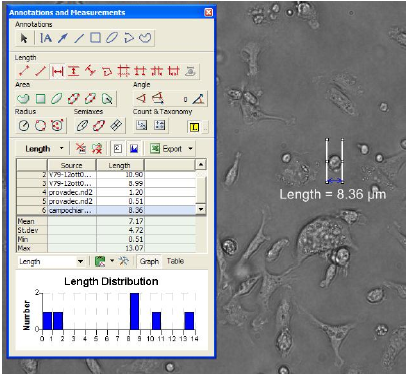
\includegraphics[scale=.60]{img/CAP2dist.png}
 \caption{\small{Esempio di utilizzo del software Nis-Element 3.1 per misure di distanza.}}
 \label{fig:dist}
\end{figure}

\begin{figure}
 \centering
 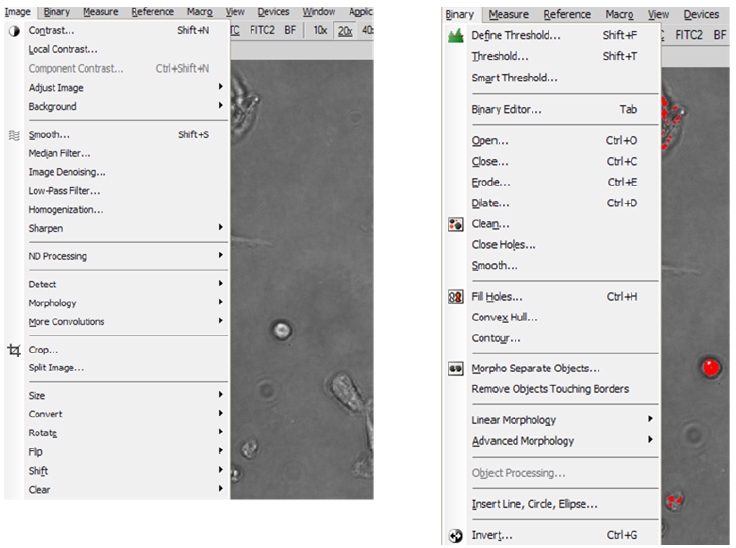
\includegraphics[scale=.40]{img/CAP2elab.png}
 \caption{\small{Panoramica di alcune operazioni di elaborazione di immagini previste dal software Nis-Element 3.1.}}
 \label{fig:elab}
\end{figure}


\section{Imperfezioni e difetti dell'immagine}

Nel campo dell'ottica, data la complessità dello studio geometrico del comportamento delle lenti, spesso ci si limita ad una trattazione basata sulla cosiddetta \textit{approssimazione di Gauss} \cite{difetti}. 
Questa teoria, detta anche ``teoria delle lenti sottili'' o ``ottica parassiale'', è applicabile per sistemi ottici ideali, ossia sistemi che soddisfano tali richieste:

\begin{itemize}
\item lenti di spessore trascurabile;

\item raggi incidenti parassiali, quindi molto prossimi all'asse della lente, e poco inclinati sull'asse, cosicchè tutti gli angoli da essi formati (es. angoli di incidenza, di apertura e di campo) siano piccoli, tali da approssimare $sin\theta \sim tan\theta$;

\item radiazione monocromatica;

\item onde sferiche o, nel caso in cui il loro raggio di curvatura  sia molto grande, piane.
\end{itemize}

Il risultato di tali ipotesi semplificative è che le immagini godono anch'esse di proprietà ideali, quali:

\begin{itemize}
\item l'immagine di un oggetto esteso, piano e perpendicolare all'asse è geometricamente simile all'oggetto e a sua volta piana e perpendicolare all'asse;

\item l'immagine di un oggetto privo di dimensioni, cioè di un punto, è ancora un punto;

\item i valori dell'ingrandimento, della focale e la posizione dei punti principali sono indipendenti dalle dimensioni dell'oggetto, dall'inclinazione dei raggi sull'asse e dalle lunghezze d'onda interessate;

\item il contrasto nell'immagine risulta uguale a quello nell'oggetto.
\end{itemize}

Ossia, sulla base dell'approssimazione di Gauss si otterrebbero immagini piane, non deformate e con risoluzione infinita, in quanto ogni punto dell'oggetto avrebbe il suo corrispondente nell'immagine e si potrebbero ritrovare in quest'ultima strutture e dettagli dell'oggetto piccoli quanto si vuole, con contrasto immutato (fino ai limiti di risoluzione del rivelatore).
Tuttavia sussistono tre cause principali di deviazione dello stato reale da quello ideale, e quindi dell'immagine effettivamente osservata da quella prevista secondo tale teoria: cause geometriche, fisiche e tecniche.
Tutte queste degradano l'immagine in vari modi, riducendone la qualità e limitando le possibilità di ottenere risultati quantitativi non distorti senza effettuare delle correzioni appropriate.

\subsection{Cause geometriche}

Quando si considerano sistemi reali di lenti spesse, con angoli di campo e di apertura non trascurabili e radiazione policromatica, risultano essere molto rilevanti per la formazione dell'immagine anche gli effetti rifrattivi sulle interfacce di riferimento (superficie aria-vetro o vetro-vetro).
Le differenze dall'immagine ideale causate da tale classe di deviazioni dalle condizioni ideali dell'ottica di Gauss sono globalmente indicate con il termine di \textit{aberrazioni}.

Il loro effetto globale è la produzione, per ogni punto oggetto, di un'immagine allargata, detta ``cerchio di confusione'', di forma e profilo fotometrico assai variabile. 
Tale cerchio danneggia sia la risoluzione dell'immagine che il microcontrasto, dove con tale termine si intende l'andamento fotometrico dell'immagine di un oggetto in cui una zona buia ed una luminosa sono separate da una linea netta, senza transizioni. 
Infatti, a causa della presenza del cerchio di confusione il passaggio chiaroscuro all'interno dell'immagine non è più rappresentabile con una curva a gradino, bensì avente pendenza più o meno regolare, comportando perciò una minor definizione (o nitidezza) dell'immagine stessa.

Le aberrazioni del punto possono essere di diverso tipo:
\begin{enumerate}
 \item aberrazione cromatica;
 \item aberrazione sferica;
 \item coma;
 \item astigmatismo;
 \item distorsione.
\end{enumerate}


\subsubsection*{Aberrazione cromatica}
L'aberrazione cromatica è legata alla lunghezza d'onda della radiazione osservata e perciò risulta assente per radiazione di tipo monocromatico. 
Ai fini della microscopia a fluorescenza, l'aberrazione cromatica risulta essere non trascurabile all'aumentare del numero di fluorofori differenti utilizzati all'interno del campione.

\begin{figure}
 \centering
 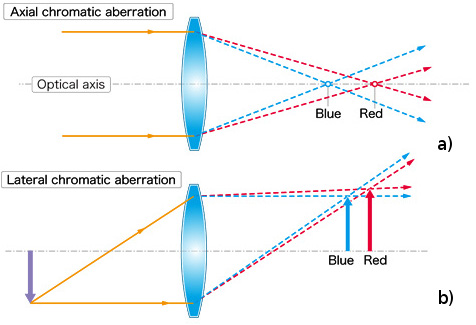
\includegraphics[scale=.60]{img/CAP2ac.jpg}
 \caption{\small{Formazione dell'aberrazione cromatica longitudinale (caso a) e trasversale (caso b).}}
 \label{fig:ac}
\end{figure}

Per la comprensione di tale fenomeno si supponga di utilizzare radiazione bianca per la formazione dell'immagine, così da disporre di un intero spettro continuo entro il range del visibile, ossia circa [400-800] nm. Ad ognuna delle lunghezze d'onda $\lambda$ interne a tale intervallo sarà associato un determinato indice di rifrazione $n$, secondo la legge di Cauchy \cite{nigro}:
$$n(\lambda) = A + \frac{B}{\lambda ^2}$$
dove A e B sono costanti dipendenti dal mezzo in esame.
Questo comporta un diverso angolo di deviazione, angolo tra la direzione entrante ed uscente del raggio, dato che, tramite costruzione geometrica, risulta direttamente proporzionale all'indice stesso.

Tale variazione dell'angolo di dispersione, quindi della focale, al variare della lunghezza d'onda provoca una variazione della coniugata immagine, dando origine alla cosiddetta \textit{aberrazione cromatica assiale o longitudinale}. 
Per tale effetto, un oggetto che emette o è attraversato da luce bianca fornisce una serie di sue immagini di differente colore, a diversa distanza dalla lente: la distanza massima si avrà per le lunghezze d'onda maggiori (parte rossa del visibile) poiché corrispondenti ad indice di rifrazione minore e quindi focale maggiore (\figurename~\ref{fig:ac}/a). 
Si ha dunque una successione di immagini corrispondenti ai valori di lunghezza d'onda presenti, detta ``spettro primario'' e l'immagine risultante appare quindi circondata da aloni colorati (\figurename~\ref{fig:aca}).

\begin{figure}
 \centering
 
\includegraphics[scale=.88]{img/CAP2aca.jpg}
 \caption{\small{Esempio di aberrazione cromatica assiale.}}
 \label{fig:aca}
\end{figure}

Supponiamo a questo punto di ignorare o di avere corretto la cromatica assiale e quindi che la posizione focale dell'immagine sia unica per tutto lo spettro.
Ciò nonostante, la dispersione dell'indice di rifrazione e della focale portano ad un diverso ingrandimento per ogni valore di lunghezza d'onda (\figurename~\ref{fig:ac}/b). 
Questo significa, sempre operando in luce bianca, che le infinite immagini possono anche giacere sullo stesso piano, ma hanno diverse dimensioni (\figurename~\ref{fig:acl}). 
Tale effetto viene definito con il nome di \textit{aberrazione cromatica laterale o trasversale}.
In tal caso gli aloni non esistono al centro del campo e crescono di larghezza all'aumentare della distanza dall'asse, cioè del campo stesso.

\begin{figure}
 \centering
 
\includegraphics[scale=.40]{img/CAP2acl.jpg}
 \caption{\small{Aberrazione cromatica laterale della Luna.}}
 \label{fig:acl}
\end{figure}

Per ridurre la cromatica assiale si possono combinare vetri con diverso potere dispersivo, così da ottenere sistemi convergenti o divergenti in cui i valori di focale e di immagine coniugata coincidono per due lunghezze d'onda agli estremi dello spettro visibile. 
In ordine del grado di complessità crescente e del numero di lenti utilizzate nel sistema, si hanno le cosiddette correzioni acromatiche ed apocromatiche, associate ai corrispondenti obiettivi acromatici ed apocromatici. 
Inoltre il diametro del suo cerchio di confusione diminuisce chiudendo il diaframma d'apertura. 
Tale aberrazione dipende molto dalla combinazione dei sistemi ottici (obiettivo, oculare e sistemi intermedi) e può essere ridotta tramite l'uso di filtri. 
Per quanto riguarda la cromatica laterale, la larghezza delle frange colorate prodotte non dipende dall'apertura del diaframma.
Ancor più della longitudinale, questa cromatica è sensibile all'accoppiamento obiettivo-oculare, alla presenza di sistemi intermedi ed all'uso di filtri.

\subsubsection*{Aberrazione sferica}
L'aberrazione sferica è un'aberrazione del punto di tipo acromatico, ossia presente anche con radiazione monocromatica, pur essendo il suo andamento legato al valore della lunghezza d'onda in gioco.
L'aberrazione sferica è una variazione della focale e quindi della posizione dell'immagine al variare dell'apertura. 

\begin{figure}
 \centering
 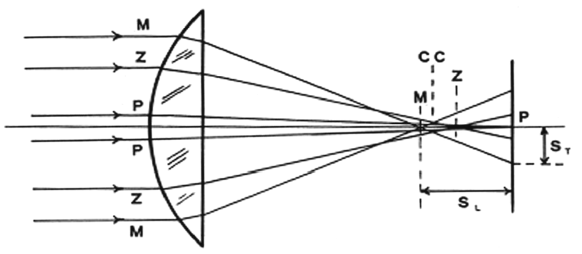
\includegraphics[scale=.50]{img/CAP2as.png}
 \caption{\small{Formazione dell'aberrazione sferica.}}
 \label{fig:as}
\end{figure}

La \figurename~\ref{fig:as} illustra il fenomeno nel caso particolare di distanza infinita del punto dalla lente: per uno stesso punto oggetto si hanno diverse immagini a diversa distanza dalla lente al variare dell'apertura, ossia dell'inclinazione, degli infiniti raggi convergenti nell'immagine.
Si identificano un fuoco ``parassiale'' P formato alla minima apertura, un fuoco ``marginale'' M alla massima apertura ed uno ``zonale'' Z formato da raggi appartenenti ad una regione intermedia.
Qualunque dei fuochi sopra citati si scelga come migliore immagine, esso sarà sempre circondato da un alone dovuto ai raggi che convergono in un fuoco più vicino o più lontano (\figurename~\ref{fig:sfer}). Questo alone è sempre presente e si può solamente cercare di minimizzarlo. 

\begin{figure}
 \centering
 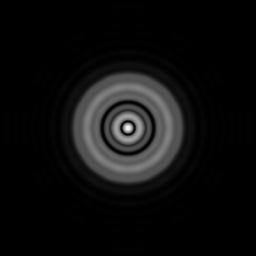
\includegraphics[scale=.55]{img/CAP2sfer.jpg}
 \caption{\small{Esempio di aberrazione sferica su un punto oggetto.}}
 \label{fig:sfer}
\end{figure}

L'inviluppo di tutti i raggi appartenenti a tutte le zone della lente costituisce una figura caratteristica, detta ``caustica'', che, sezionata con un piano perpendicolare all'asse, mostra sempre una figura circolare, mai un punto.
\'E proprio la caustica che rappresenta il cerchio di confusione dovuto all'aberrazione sferica e si cercherà sempre il cerchio di minima confusione, (CC in \figurename~\ref{fig:as}), dato che tale figura si può minimizzare cercando il miglior fuoco, ma mai annullare.

Il termine ``sferica'' si riferisce al fatto che tale aberrazione è legata alla forma sferica delle superfici delle lenti usuali e perciò si può eliminare dando forme asferiche particolari, metodo utilizzato per collettori, condensatori e certi obbiettivi fotografici, oppure combinando lenti sferiche di forma ed indice diversi, metodo utilizzato nei microscopi. 
Un sistema corretto dall'aberrazione sferica si chiama aplanatico.

\subsubsection*{Coma}
La coma ha come radice etimologica i termini ``chioma'', ``cometa'', facendo riferimento al suo tipico aspetto, ancor più evidente se agente su piccoli oggetti (\figurename~\ref{fig:coma}).

\begin{figure}
 \centering
 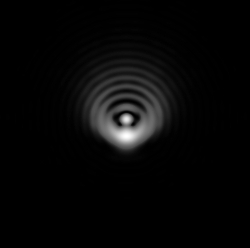
\includegraphics[scale=.55]{img/CAP2coma.jpg}
 \caption{\small{Esempio di coma su un punto oggetto.}}
 \label{fig:coma}
\end{figure}

Questa aberrazione acromatica è di tipo extra-assiale, così come la cromatica laterale, ossia non esiste sull'asse di un sistema centrato e cresce con l'aumentare del campo. 
Di conseguenza il suo cerchio di confusione non può essere circolare ma risulta allungato in senso radiale e presenta un punto molto luminoso che sfuma gradatamente in una larga coda.
Questo difetto ha origine quando l'oggetto osservato non è allineato con l'asse di osservazione.

In microscopia la coma si corregge facilmente scegliendo in modo opportuno la posizione del diaframma e la forma delle lenti, prestando attenzione al fatto che essa è assente in un sistema simmetrico col diaframma al centro.
Risulta ovvio che la coma in asse non può esistere, perciò se al centro del campo di un microscopio si osserva un residuo di coma in generale è indice che una o più lenti dell'obiettivo non sono centrate sull'asse comune.

\subsubsection*{Astigmatismo}
L'astigmatismo è un'aberrazione acromatica, extra-assiale che crea un'immagine sdoppiata e deformata di ogni punto oggetto (\figurename~\ref{fig:astigmatismo}). In tal caso, il fascio di raggi che convergono nell'immagine di un punto oggetto non si raccoglie attorno ad una zona circolare, bensì attorno ad un segmento tangenziale, detto ``focale astigmatica''.
Questo è dovuto ad un differente fuoco per angoli di rotazione intorno all'asse ottico.
Un fascio conico a sezione circolare viene quindi deformato in uno non circolare in seguito alla diversa focale che i raggi hanno.

\begin{figure}
 \centering
 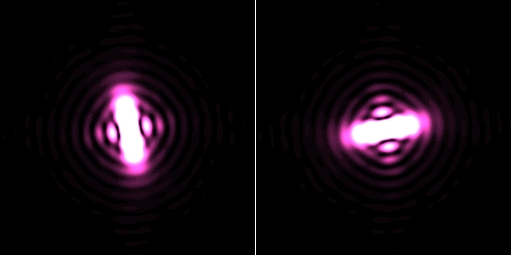
\includegraphics[scale=.50]{img/CAP2astig.jpg}
 \caption{\small{Esempi di astigmatismo su un punto oggetto.}}
 \label{fig:astigmatismo}
\end{figure}

L'astigmatismo, come la coma, è nullo sull'asse e cresce col campo. 
Se nell'uso pratico si riscontra astigmatismo anche al centro del campo allora le cause possono essere varie: inclinazione di qualche prisma o di qualche lente rispetto all'asse, errore di centratura o errore nella forma di qualche lente.
Tuttavia modificando la messa a fuoco del microscopio, si evince una grande differenza tra la figura della coma e dell'astigmatismo nell'immagine di un punto oggetto: la prima si può allargare ma conserva la sua forma, con la coda che resta diretta radialmente, mentre la seconda si allunga in direzione da radiale a tangenziale o viceversa. 

Per la correzione di tale aberrazione bisogna tener conto che essa è influenzata, più che dalla forma delle lenti, dalla posizione del diaframma e dal numero di lenti interposte, dato che una lente divergente mostra un astigmatismo di segno opposto di una convergente, da cui l'utilità di porne varie in successione. 
Un sistema corretto da astigmatismo si chiama genericamente ``anastigmatico''. 

\subsubsection*{Distorsione}
La distorsione consiste in una variazione dell'ingrandimento trasversale con la distanza dall'asse, per cui l'immagine di un oggetto esteso piano non gli è simile. 
Se l'ingrandimento cresce col campo, cioè con la distanza del punto dall'asse, allora l'oggetto sembra dilatarsi verso la periferia e si parla di distorsione positiva o ``a cuscinetto''; viceversa, se l'ingrandimento diminuisce al crescere del campo allora l'oggetto sembra contrarsi e si ha la cosiddetta distorsione negativa o ``a barilotto'' (\figurename~\ref{fig:distorsione}).

\begin{figure}
 \centering
 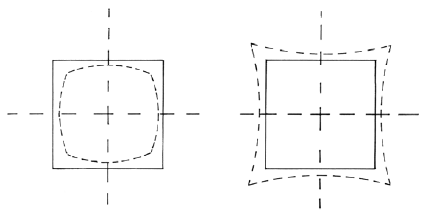
\includegraphics[scale=.65]{img/CAP2disto.png}
 \caption{\small{Distorsione a barilotto (sinistra) e a cuscinetto (destra) di un oggetto quadrato.}}
 \label{fig:distorsione}
\end{figure}

La distorsione di una lente sottile è in genere trascurabile, non è invece così per le lenti spesse: una lente spessa convergente tende a mostrare una distorsione positiva, se invece divergente la mostra negativa.
Tuttavia in microscopia la distorsione disturba i fini dell'esperimento solo quando si debbono eseguire misure di superficie o di lunghezza sull'oggetto, ma in genere essa è assai contenuta ed in prevalenza data dall'oculare poichè quella dell'obbiettivo non supera in genere l'1\%.
Un sistema corretto da distorsione e curvatura di campo si dice ortoscopico.


\subsection {Cause fisiche}

Finora abbiamo esaminato molti fenomeni ottici, che si verificano nel microscopio, servendoci di un approccio per lo più di natura geometrica e si è visto in tale contesto che, dato un punto oggetto, un sistema ottico reale non produce mai un'immagine puntiforme, se non altro a causa delle aberrazioni del punto.
Supponendo ora di operare in un sistema ideale, in cui siano assenti sia le aberrazioni che i difetti costruttivi, ebbene nuovamente non riusciremo ad ottenere da esso un'immagine puntiforme. 
Ciò è dovuto al fatto che la radiazione elettromagnetica non si può trattare sempre come se costituita da semplici ``raggi'', ossia rette di propagazione che obbediscono solo a leggi geometriche, bensì è necessario tenere conto della sua natura ondulatoria.
Una tipica conseguenza che si evince da tale approccio fisico alla propagazione della radiazione è la generazione di effetti diffrattivi.

Per comprendere tale fenomeno consideriamo una sorgente puntiforme Q, posta davanti ad uno schermo avente una fenditura circolare P, con una lente convergente L posta a ridosso dell'apertura, che crea sullo schermo S l'immagine Q' dell'oggetto Q (\figurename~\ref{fig:diff}).
Si noti l'evidente analogia che intercorre tra la fenditura P ed un diaframma d'apertura per la lente L.

\begin{figure}
 \centering
 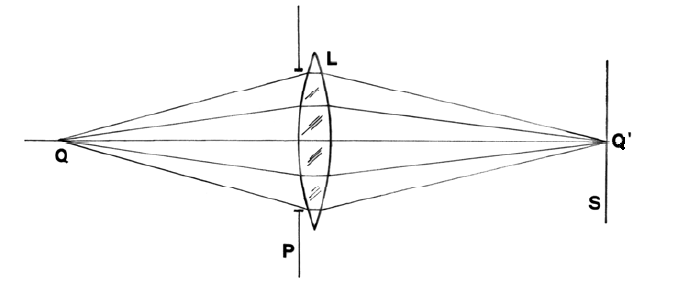
\includegraphics[scale=.55]{img/CAP2diff.png}
 \caption{\small{Schema del sistema fenditura-lente convergente per la formazione della figura di diffrazione.}}
 \label{fig:diff}
\end{figure}

Supponendo che la lente sia stata corretta da ogni tipo di aberrazione, il cerchio di confusione è previsto con raggio nullo. 
In realtà ciò che si osserva in Q' è una figura caratteristica, detta \textit{figura di diffrazione}, o anche ``figura di Airy'' o ``centrica'', avente l'aspetto tipico mostrato dalla \figurename~\ref{fig:diff2}: un disco centrale di massima intensità con orli sfumati (``disco di Airy''), circondato da una successione di anelli concentrici scuri e chiari, sempre sfumati e di intensità decrescente.

\begin{figure}
 \centering
 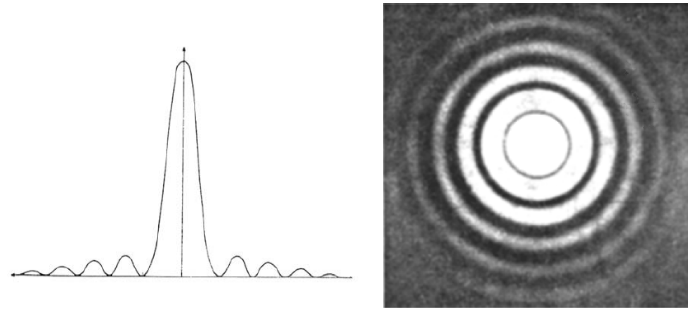
\includegraphics[scale=.55]{img/CAP2diff2.png}
 \caption{\small{Profilo fotometrico della centrica (sinistra) e figura di Airy (destra).}}
 \label{fig:diff2}
\end{figure}

Detta $NA$ l'apertura numerica della lente L e $\lambda$ la lunghezza d'onda dell'onda incidente, i valori del raggio dell'ennesimo anello chiaro sono:
$$r_n = k_n \frac{\lambda}{NA} $$
dove $k_n$ vale 0.61, 1.12 e 1.62 rispettivamente per il primo (disco di Airy), secondo e terzo anello chiaro.
\'E inutile andare oltre poiché gli anelli successivi sono troppo poco intensi per poter essere osservati, dato che l'intensità decresce molto rapidamente nelle varie zone della centrica. 
Infatti per il  disco di Airy l'energia è l'84\% di quella totale e per i successivi anelli: 7,1\%, 2,8\% e 1,5\%.

Dunque, un sistema ottico ideale, anche in assenza di aberrazioni, non dà un'immagine puntiforme di un punto oggetto, ma nuovamente una sorta di cerchio di confusione, questa volta non dovuto a fenomeni geometrici, quali la rifrazione, ma a fenomeni ondulatori, cioè alla diffrazione.

L'effetto diffrattivo, al contrario delle aberrazioni, è una proprietà intrinseca alla natura fisica del fenomeno in esame e perciò è molto più difficile poter limitare i difetti da esso apportati sull'immagine. 
Tuttavia, in alcuni casi, esso può venire attenuato tramite algoritmi applicati in una fase post-acquisizione sull'immagine desiderata, come per esempio con il cosiddetto \textit{algoritmo di deconvoluzione}.
Questa  tecnica inizialmente nacque con lo scopo di rimuovere le sfocature caratteristiche di un sistema fuori fuoco che contaminavano le immagini di una vasta gamma di microscopi \cite{decon}. 

\begin{figure}
 \centering
 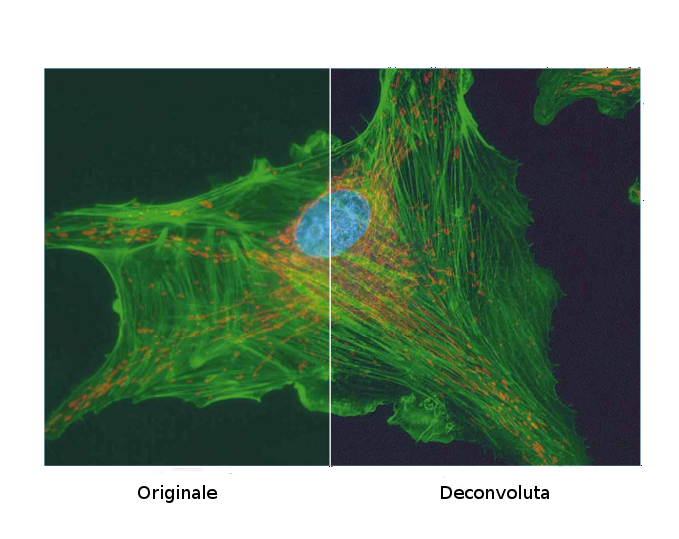
\includegraphics[scale=.60]{img/CAP2decon.png}
 \caption{\small{Immagine a fluorescenza di una cellula endoteliale di bovino. La regione a sinistra mostra l'immagine originale, quella a destra il risultato di un processo iterativo di deconvoluzione bidimensionale.}}
 \label{fig:decon}
\end{figure}

Un microscopio è in genere caratterizzato dalla sua ``Point Spread Function'' (PSF), una descrizione bidimensionale o tridimensionale di come un singolo punto luce venga trasformato dallo strumento e mostrato all'utilizzatore. 
La PSF è determinata dalla combinazione delle caratteristiche ottiche del campione, del vetrino, delle lenti dell'obiettivo e della lunghezza d'onda usata; per esempio un microscopio confocale ha tipicamente una PSF che assomiglia ad un ellissoide posto nella direzione assiale.
Un oggetto arbitrario può essere pensato come insieme di punti luce posti in diverse posizioni, con differenti intensità. 
Quindi, l'immagine osservata dall'utilizzatore può essere descritta come una sovrapposizione di varie PSF, ciascuna nella posizione del corrispondente punto luce all'interno del campione, con intensità opportunatamente scalata.
Matematicamente tale operazione è detta ``convoluzione'', perciò, invece che vedere un'immagine pulita, si osserva, a causa della sovrapposizione delle PSF, una sfocatura che copre le caratteristiche di interesse. 
Di conseguenza l'immagine ottenuta dal microscopio non è una rappresentazione fedele dell'oggetto in esame, bensì una semplice rappresentazione di esso.
L'operazione necessaria per correggere questa ``sfocatura'' è detta deconvoluzione, in quanto corrisponde all'operazione inversa della convoluzione che ha dato origine all'immagine.
Lo scopo della deconvoluzione è proprio utilizzare la rielaborazione via software per invertire tale processo e ripristinare l'immagine fedele dell'oggetto in esame. 
Questo particolare algoritmo sta diventando negli ultimi anni parte integrante della microscopia digitale poiché, come si evince dalla \figurename~\ref{fig:decon}, è in grado di produrre immagini rielaborate con maggior risoluzione, miglior contrasto e rapporto segnale-rumore più elevato.

\subsection {Cause tecniche} 

L'immagine acquisita con il microscopio può essere affetta da difetti non solo di natura fisica-geometrica ma anche di origine tecnica-strumentale. 
In linea di principio si tratta di difetti eliminabili con opportuni accorgimenti tecnici, generalmente con un certo aggravio di costi di produzione e manutenzione.

Essi possono essere legati ad una imprecisa lavorazione dei materiali presenti all'interno del microscopio, come per esempio: irregolarità delle superfici, difetti nell'omogeneità dei materiali trasparenti, luce diffusa sulle pareti o sulle montature delle lenti, difetti di montaggio e di centratura, errori di messa a fuoco e mancata pulizia.

D'altra parte si può trattare anche di difetti intrinseci alla misura stessa, come ad esempio la presenza di una fluorescenza residua di sfondo e la non omogeneità del fascio. 
Entrambe sono connesse alla luce di eccitazione utilizzata durante l'esperimento: la prima inserisce un offset di luminosità nel background dell'immagine, mentre la seconda crea immagini con, a priori, intensità differente a seconda della posizione del pixel preso in esame, causate da un fascio di radiazione di per sé non omogeneo.




\clearpage{\pagestyle{empty}\cleardoublepage}

\chapter{Algoritmo di correzione dell'immagine}

\begin{flushright}\begin{small}\textit{"Any fool can write code that a computer can understand.\\
Good programmers write code that humans can understand."}\\
- Martin Fowler -\\
\end{small}\end{flushright}

Questo capitolo descrive il software sviluppato per l'elaborazione di immagini all'interno del progetto di tesi, esplicitando l'approccio statistico ed algoritmico utilizzato.

L'algoritmo, scritto nel linguaggio di programmazione Python \cite{python}, ha lo scopo di ``ripulire'' le immagini acquisite col microscopio a fluorescenza da alcuni difetti di natura tecnico-sperimentale, connessi perlopiù alla sorgente di luce dello strumento (capitolo 2.2.3). 
In particolare le correzioni apportate all'immagine sono mirate all'eliminazione delle distorsioni presenti ai bordi del campo rilevato e della fluorescenza di background. 
Infatti, come si evince dalla \figurename~\ref{fig:bordi}, ogni immagine a fluorescenza è inevitabilmente affetta da una luminosità residua di sfondo, causata dalla necessità di una sorgente di luce per l'eccitazione del campione, e da una luminescenza disomogenea, intrinsecamente connessa all'irregolarità spaziale dell'illuminazione della sorgente.
Quest'ultimo difetto è quello che grava maggiormente su un'eventuale analisi quantitativa dell'immagine e, poiché ineliminabile dal punto di vista pratico-operazionale, è possibile affrontarlo unicamente tramite un'elaborazione via software. 

\begin{figure}
 \centering
 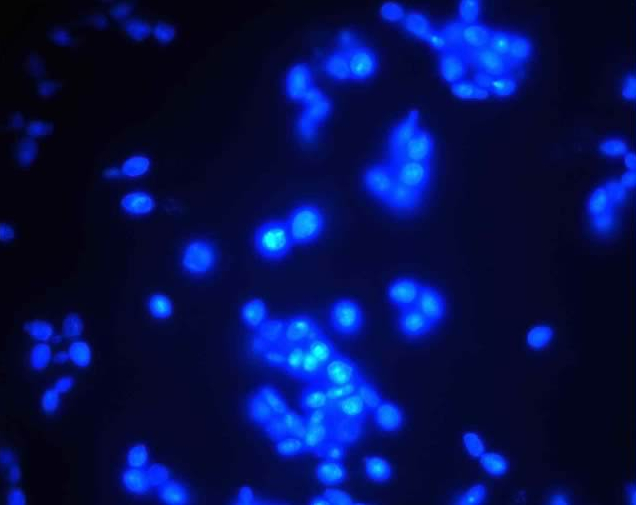
\includegraphics[scale=.55]{img/CAP3bordi.jpg}
 \caption{\small{Immagine in colorazione DAPI di cellule di lievito osservate al microscopio a fluorescenza: ben evidente la disomogeneità spaziale della luminescenza e la presenza di una luminosità residua di sfondo.}}
 \label{fig:bordi}
\end{figure}

Questo programma di correzione della luminosità sfrutta delle sfere nanometrice, di dimensione costante ed intensità di luminosità nota, prodotte appositamente per la calibrazione dei microscopi a fluorescenza.
Esistono diversi set di nanosfere in grado di coprire ampi range di intensità, così da poter creare una curva di calibrazione dall'intensità del segnale osservato (dipendente ad esempio dalla luminosità dell'irraggiamento e dal tempo di esposizione) alla concentrazione di fluoroforo sottostante.
 
Nel nostro caso si è sfruttato il kit di sfere nanometriche fluorescenti nel rosso ``InSpeck Microscope Image Intensity Calibration'', acquistate appositamente per la calibrazione del microscopio in uso.
Esso consiste in una fiala di $5\ ml$ di mezzo di sospensione e 7 fiale di microsfere di polistirene atossico aventi differenti intensità relative: 0\%, 0.3\%, 1\%, 3\%, 10\%, 30\% e 100\%.
Tale richiesta nasce dal fatto che l'algoritmo effettua la correzione dell'immagine a fluorescenza delle cellule sfruttando l'ulteriore acquisizione di due immagini di calibrazione: una di sferette aventi stessa intensità e l'altra di sferette con 5 intensità distinte.

Descriviamo dunque passo a passo le fasi principali dell'algoritmo, riportato nella sua interezza in Appendice A, che possono essere schematizzate in:
\begin{enumerate}
 \item rimozione delle disomogeneità ai bordi dell'immagine,
 \item rimozione della fluorescenza di background,
 \item correzione dell'immagine bersaglio.
\end{enumerate}


\section{Rimozione delle disomogeneità di illuminazione}

Come precedentemente osservato, la disomogeneità di illuminazione comporta immagini a microscopia a fluorescenza con maggior segnale luminoso nella zona centrale rispetto alle regioni periferiche.
L'algoritmo mira alla compensazione di questa disomogeneità stimando punto per punto il valore di segnale atteso a parità di concentrazione di fluoroforo ed usando questa stima per correggere le stime osservate.
Per far questo necessita di una immagine di calibrazione, ossia di un campo contenente solo nanosfere con un'unica intensità (\figurename~\ref{fig:unaint}).
Tramite questa calibrazione l'algoritmo riesce a eliminare in modo sostanziale la dipendenza dell'intensità dalla posizione del pixel. 

\begin{figure}[p]
 \centering
 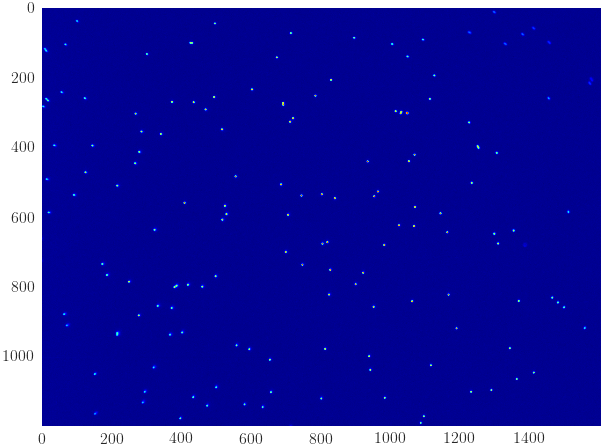
\includegraphics[scale=.64]{img/CAP3unaint.png}
 \caption{\small{Immagine a fluorescenza (1600x1200 pixel) di sferette con intensità relativa del 10\%.}}
 \label{fig:unaint}
\end{figure}

Inizialmente il programma applica sull'immagine il filtro gaussiano, tipico filtro di smoothing molto efficace per attenuare il rumore presente (counting noise dovuto alla bassa intensità delle immagini), e calcola in un primo modo approssimato l'intensità costante residua.
Questo background viene valutato in modo statistico come massimo delle mode, ossia dei valori che compaiono più frequentemente, di ogni riga della matrice bidimensionale che costituisce l'immagine. 
Tale parametro viene quindi sottratto a quest'ultima poiché valore costante in grado di alterare considerazioni quantitative.

Una volta rimossa la componente principale dello sfondo, viene stimato il campo di illuminazione incidente, supposto proporzionale al segnale di ciascuna sferetta (che dovrebbe essere altrimenti omogeneo).
Suddetto campo viene stimato tramite il fit, svolto all'interno del codice dalla routine \textit{analyze}, di una funzione pseudo-gaussiana.
Quest'ultima descrive ragionevolmente bene la luminosità osservata e di conseguenza viene usata come campo di luminosità incidente per la correzione del segnale osservato.


\subsubsection*{Ricerca dei massimi}

Il primo step necessario alla stima della funzione di illuminazione è la ricerca delle nanosfere nell'immagine.
Quest'ultime sono approssimabili come punti di luminosità diffusa, distribuiti in modo gaussiano intorno al punto centrale.
Tali luminosità vengono ipotizzate tutte proporzionali all'intensità luminosa e la possibilità che alcuni di questi punti luce siano in realtà la sovrapposizione di più sfere in contatto viene gestita nel momento del fit.

La ricerca dei massimi viene svolta dalla routine \textit{find\_max}, che prende in input tre parametri: \textit{vicinanza\_size}, \textit{soglia} e \textit{margine}.
Il primo (\textit{vicinanza\_size}) dà la dimensione in pixel dell'area sfruttata dai filtri per la ricerca dei massimi e dei minimi relativi, perciò dovrà assumere valori minori al crescere della concentrazione delle sferette, ma approssimativamente simili al diametro delle nanosfere nell'immagine. 
Il secondo (\textit{soglia}) indica quale debba essere il minimo valore di cui il massimo individuato debba superare il valore del background nei dintorni, per evitare di includere nel conteggio dei massimi dati da effetti di rumore.
Di conseguenza tale parametro dipende dalla luminosità delle sferette: maggiore sarà quest'ultima e maggiore dovrà essere il suo valore.
Dalla ricerca dei massimi viene escluso, successivamente alla determinazione dei punti di massimo (localizzazione ed intensità di ciascuna nanosfera), il confine dell'immagine, utilizzando il parametro \textit{margine}.
Esso indica la larghezza in pixel del bordo da rimuovere dalla stima, così da evitare di includere immagini parziali di nanosfere che potrebbero distorcere il fit.
Difatti ogni sferetta non viene rappresentata come punto oggetto, bensì con un cerchio di confusione (capitolo 2.2.1) e di conseguenza, nel caso in cui l'alone sia a cavallo del margine dell'immagine, potrebbe venire riconosciuto come massimo un punto che in realtà non è il centro della sferetta ma un pixel della sfumatura circostante.

Sempre all'interno di \textit{find\_max} viene associata ad ogni punto di massimo un'intensità integrale media. 
Questa viene calcolata richiamando la funzione \textit{intensity}, la quale somma i valori dei pixel che costituiscono la sferetta e divide il tutto per il numero totale di pixel contati, così da tener conto del fatto che non si tratta di un punto oggetto privo di dimensioni, bensì di un'area con una certa estensione. 
Per fare ciò ovviamente è necessario valutare il raggio \textit{delta} della sferetta, nel nostro caso stimato pari a 5 pixel (\figurename~\ref{fig:punto}).

\begin{figure}
 \centering
 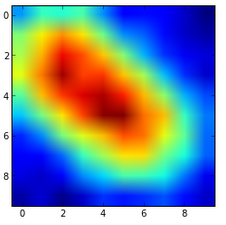
\includegraphics[scale=.25]{img/CAP3punto.png}
 \caption{\small{Selezione di una singola sferetta del kit ``InSpeck Microscope Image Intensity Calibration'' per la valutazione della dimensione associata.}}
 \label{fig:punto}
\end{figure}

\subsubsection*{Fit di maximum likelihood}

A questo punto, avendo identificato i massimi dell'immagine, si stimano i parametri della funzione di illuminazione tramite un metodo di \textit{maximum likelihood}, utilizzando un metodo pre-esistente nel modulo scipy di python, chiamato \textit{curve\_fit}.

Per poter comprendere come venga eseguita questa tipologia di fit, prendiamo un campione casuale $\mathbf{X_n}$ di $n$ osservazioni che può assumere diversi valori, ciascuno dei quali costituisce un campione osservato $\mathbf{x_n}$.
Venga inoltre definito un modello statistico per il campione $\mathbf{X_n}$, ossia una distribuzione $f_n (\mathbf{x_n};\theta)$ con $\theta \in \Theta$ parametro (o insieme di parametri) che identifica la legge di probabilità relativa all'esperimento in corso.
Sulla base di tali identificazioni si definisce funzione di verosimiglianza (likelihood function)
associata ad $\mathbf{x_{oss}}$ la funzione $L_{x_{oss}}: \Theta\longmapsto \Re_+$ tale che:
$$L_{x_{oss}}(\theta)=f_n (\mathbf{x_{oss}};\theta)=\prod_{i=1}^n f_X (x^{oss}_i;\theta) $$
dove $\mathbf{x_{oss}}=(x^{oss}_1, x^{oss}_2, ..., x^{oss}_n)$ è il campione osservato. 
La likelihood function è utilizzata solitamente per condurre tre tradizionali procedure:
\begin{itemize}
 \item ottenere una stima puntuale di $\theta$,
 \item ottenere una stima per intervallo di $\theta$,
 \item scegliere tra due possibili ipotesi riguardanti valori di $\theta$.
\end{itemize}
Il fit di maximum likelihood, utilizzato nell'algoritmo, è volto ad ottenere la stima puntuale, detta anche stima di massima verosimiglianza (MLE). 
Con tale termine si indica il valore $\hat{\theta}$ in cui la funzione di verosimiglianza raggiunge il massimo assoluto, ossia:
$$MLE = \hat{\theta}\ se\ L_{x_{oss}}(\hat{\theta})=\max_{\theta \in \Theta} L_{x_{oss}}(\theta)$$
Detto in altri termini, il punto di massimo della funzione di verosimiglianza è il valore più plausibile di $\theta$ alla luce del campione osservato $x_{oss}$.

Dopo varie analisi si è notato che la funzione che al meglio descrive il comportamento dei massimi di intensità è proporzionale ad una gaussiana multivariata, descritta all'interno della funzione \textit{gauss} tramite la relazione:
$$ G = bg + maxint \cdot \exp \bigg\{ {-\frac{1}{2} \bigg[{ (\frac{x-cx}{dsx})^2   +  (\frac{y-cy}{dsy})^2  +  \frac{corr \cdot (x-cx) \cdot (y-cy)}{dsx \cdot dsy} \bigg]}^{\frac{e}{2}}}\bigg\} $$
dove $bg$ è il parametro di background, $maxint$ è l'intensità massima, $cx$ e $cy$ sono rispettivamente i centri delle coordinate x e y, $dsx$ e $dsy$ sono rispettivamente le deviazioni standard delle coordinate x e y, $corr$ è il parametro di correlazione tra x ed y ed infine $e$ è l'esponente.
Facendo riferimento alla trattazione precedente, $G$ corrisponde alla funzione di verosimiglianza $L_{x_{oss}}(\theta)$, ove $\theta$ in tal caso è l'insieme dei parametri $(bg,\ maxint,\ cx,\ cy,\ dsx,\ dsy,\ corr,\ e)$.
Essendo questo uno dei punti cardine della correzione, si è deciso di parallelizzare la funzione \textit{gauss}, così da avere un guadagno nei tempi dell'ordine di quattro volte.

\begin{figure}
 \centering
 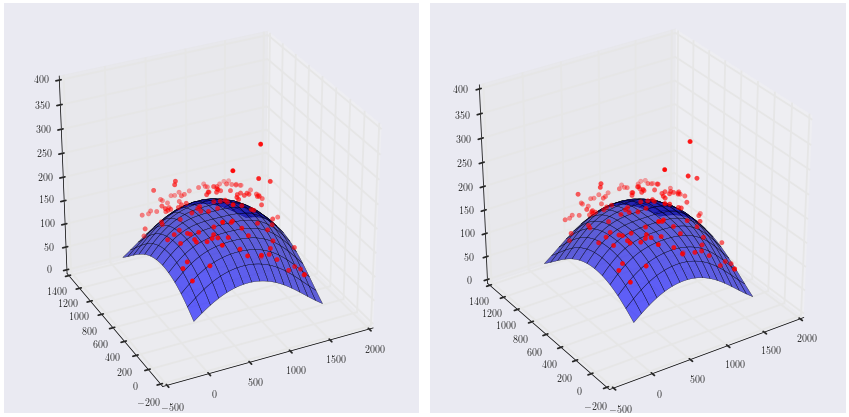
\includegraphics[scale=0.45]{img/CAP3gauss.png}
 \caption{\small{Immagine in visione ``cross eyed stereoscopic'': i puntini rappresentano i massimi della \figurename~\ref{fig:unaint} mentre la superficie è quella risultante dal fit di maximum likelihood.}}
 \label{fig:gauss}
\end{figure}

\begin{figure}[p]
 \centering
 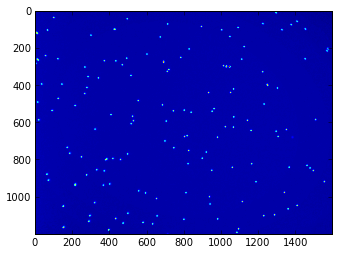
\includegraphics[scale=.64]{img/CAP3unaintcorr.png}
 \caption{\small{Immagine risultante dalla correzione della disomogeneità di campo sull'immagine in \figurename~\ref{fig:unaint}.}}
 \label{fig:unaintcorr}
\end{figure}

Una volta ottenuta la stima di massima verosimiglianza, ossia il set di parametri in grado di massimizzare la likelihood function, ciò che si viene a creare è una superficie tridimensionale con forma analoga a quella riportata in \figurename~\ref{fig:gauss}. 
Quest'ultima immagine mette bene in evidenza il fatto che alcuni punti di massimo corrispondono ad intensità molto elevate rispetto alla media, pur trattandosi di sferette con medesima intensità relativa.
Questo fenomeno è da associarsi alla possibilità che due sferette possano trovarsi così vicine da apparire sovrapposte e, essendo questa un'alterazione dei risultati, è necessario rieseguire il calcolo dei parametri dopo aver eliminato tali punti più intensi. 
Per fare ciò viene utilizzato il quantile$_{0.95}$ dei massimi normalizzati, ossia vengono eliminati dal nuovo fit quei pixel con intensità superiore ad esso, pari per definizione al 5\% dei massimi inizialmente rilevati.
I nuovi parametri ottenuti a questa seconda iterazione sono restituiti dalla funzione \textit{analyze} e sono utilizzabili per la correzione delle disomogeneità nelle regioni periferiche dell'immagine di una qualunque immagine a fluorescenza rilevata con lo stesso apparato, inclusa la stessa di calibrazione (\figurename~\ref{fig:unaintcorr}).
Infatti a questo punto, inserendo una qualsiasi immagine come variabile di ingresso della funzione \textit{correction}, è possibile eliminare tale difetto sfruttando unicamente la stima di massima verosimiglianza precedentemente calcolata. 
Tale funzione è molto semplice poiché sfrutta la normalizzazione del valore dei pixel dell'immagine sulla base del valore previsto dalla superficie tridimensionale, rinormalizzando il segnale osservato per la funzione di intensità di illuminazione ottenuta.



\section{Rimozione della fluorescenza di background}

La seconda immagine di calibrazione, costituita da nanosfere aventi differenti intensità (\figurename~\ref{fig:piuint}), viene sfruttata per correggere il problema della fluorescenza residua di sfondo, tramite il controllo della risposta lineare dello strumento. 

\begin{figure}[p]
 \centering
 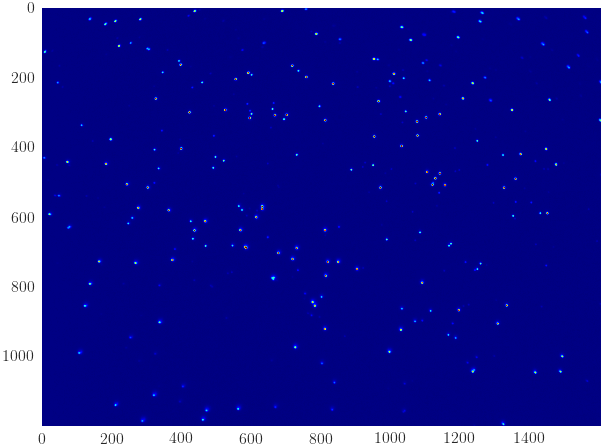
\includegraphics[scale=.64]{img/CAP3piuint.png}
 \caption{\small{Immagine a fluorescenza (1600x1200 pixel) di sferette con cinque differenti intensità relative: 1\%, 3\%, 10\%, 30\% e 100\%.}}
 \label{fig:piuint}
\end{figure}

Come nella prima fase dell'algoritmo, all'utente viene richiesto di inserire la seconda immagine di calibrazione.
A questa viene applicato uno smoothing gaussiano e sottratto il parametro del background. 
Successivamente, sulla base dei parametri del fit calcolati tramite la prima immagine di calibrazione viene corretta la disomogeneità di illuminazione.

A questo punto ai fini del controllo della risposta lineare del microscopio, vengono riconosciute nell'immagine le curve gaussiane relative alle differenti intensità. 
Nel nostro caso sono stati inseriti nel campione cinque diversi tipi di sferette, escludendo quelle con intensità relativa del 0.3\% poiché non sufficientemente intensa intensa, e di conseguenza vengono riconosciute cinque distinte curve gaussiane.
Queste sono state identificate tramite un \textit{Gaussian Mixture Model (GMM)} sul logaritmo delle intensità, nel quale le intensità sono distribuite in modo approssimativamente regolare con deviazione standard e numero di osservazioni simili fra le varie gaussiane. 
Di ciascuna di questa viene registrata la media, la deviazione standard e la numerosità.
Il fit è stato effettuato tramite la funzione per le \textit{Gaussian Mixture Model (GMM)} presente nella libreria \textit{scikits-learn}.
Un esempio dell'istogramma delle intensità risultante e del relativo fit si può vedere in \figurename~\ref{fig:istogauss}.

\begin{figure}
 \centering
 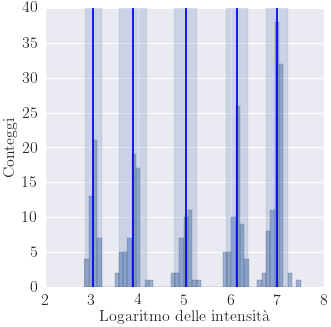
\includegraphics[scale=.60]{img/CAP3istogauss.png}
 \caption{\small{Istogramma delle cinque curve gaussiane corrispondenti alle intensità dei massimi presenti nella seconda immagine di calibrazione, una volta corretta dalla disomogeneità di illuminazione. La linea marcata e l'area sfumata presenti su ogni curva rappresentano rispettivamente il valore medio e la deviazione standard della gaussiana, identificati dalla GMM.}}
 \label{fig:istogauss}
\end{figure}

I valori medi delle gaussiane rappresentano le intensità medie di ciascuna categoria di sferette e di conseguenza, essendo queste comunque note a priori, è possibile creare una regressione lineare tra le intensità previste e quelle effettivamente rilevate all'interno del campione, così da controllare la linearità della risposta e correggere di conseguenza il parametro di background. 
Un primo fit lineare è stato fatto sfruttando la funzione \textit{linregress}, la quale restituisce un array contenente in particolare la slope e l'intercetta della curva di fit e la correlazione esistente tra i due set di dati in esame.
Come si evince dalla \figurename~\ref{fig:linearita}, la relazione tra intensità rilevate e note sembra non essere perfettamente lineare. Infatti il grafico in scala logaritmica presenta una slope non identicamente unitaria, pari a 0.87, e quello in scala lineare mostra una leggera curvatura dell'andamento dei dati. 
Inoltre le incertezze associate ai dati in esame, sebbene riportate nel grafico, risultano impercettibili, ulteriore indice del fatto che questa  difformità dalla linearità non è frutto del caso.
Ad ogni modo la discrepanza risulta essere non troppo evidente e trattabile con una trasformazione non lineare semplice dell'intensità dell'immagine; per tale motivo, in prima approssimazione, possiamo ignorare eventuali non-linearità e considerare perciò verificata l'ipotesi di risposta lineare del microscopio. 

\begin{figure}
 \centering
 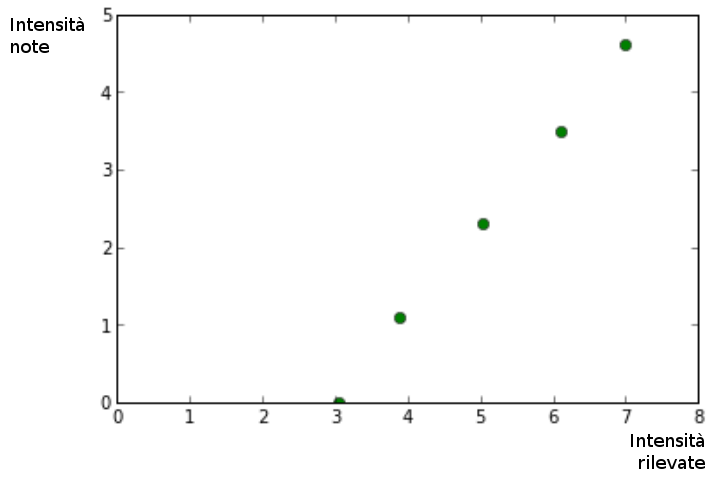
\includegraphics[scale=.55]{img/CAP3linearita.png}
 \caption{\small{Grafico con incertezze (non percettibili) delle intensità medie delle cinque gaussiane corrispondenti ai massimi della seconda immagine di calibrazione corretta dalla disomogeneità di illuminazione in funzione di quelle note ed associate rette di regressione lineare. Sulla sinistra è riportato il grafico in scala logaritmica, mentre sulla destra in scala lineare.}}
 \label{fig:linearita}
\end{figure}


\begin{figure}[p]
 \centering
 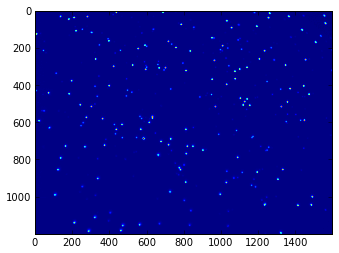
\includegraphics[scale=.64]{img/CAP3piuintcorr.png}
 \caption{\small{Immagine risultante dalla correzione della disomogeneità di illuminazione e della fluorescenza di background sull'immagine in \figurename~\ref{fig:piuint}.}}
 \label{fig:piuintcorr}
\end{figure}

Sulla base di tale ipotesi l'unico obiettivo rimasto risulta essere la rimozione del valore costante della fluorescenza di sfondo. 
Per fare ciò basta occorre traslare i valori in modo da ottenere il passaggio della retta di regressione dall'origine, ossia a livello pratico è necessario sottrarre all'immagine l'intercetta calcolata. 
Essendo questo un altro pasaggio cardine dell'algoritmo, si è scelto di rivalutare l'intercetta all'origine in modo più preciso, ossia tramite un secondo fit lineare eseguito con un'apposita funzione di \textit{curve\_fit}.
A questo punto per la rimozione della fluorescenza di background basterà semplicemente sottrarre il parametro dell'ordinata all'origine all'intera immagine presa in considerazione. 
L'immagine di calibrazione usata per correggere questo secondo difetto può essere a sua volta autocorretta, come mostrato in \figurename~\ref{fig:piuintcorr}.

Tramite questa seconda fase, che sfrutta l'immagine di calibrazione di nanosfere con differenti intensità e i parametri del fit di maximum likelihood ottenuti nella prima fase, si riesce quindi a eliminare in modo sostanziale l'ulteriore difetto della fluorescenza residua. 


\section{Correzione dell'immagine}

La parte finale del programma è volta alla correzione di entrambi i difetti, l'illuminazione disomogenea e la fluorescenza residua, per una qualsiasi immagine acquisita con il microscopio a fluorescenza (\figurename~\ref{fig:cell}). 

\begin{figure}[p]
 \centering
 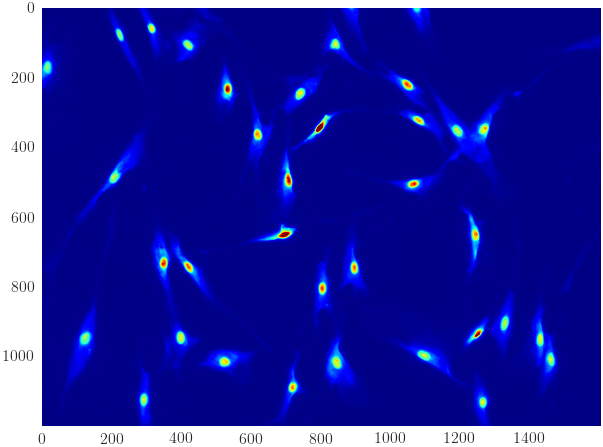
\includegraphics[scale=.64]{img/CAP3cell.png}
 \caption{\small{Immagine a fluorescenza di fibroblasti primari. Si può notare come i nuclei presenti al centro dell'immagine risultino più intensi (maggior componente rossa) rispetto a quelli vicini alla periferia.}}
 \label{fig:cell}
\end{figure}

A questo punto l'algoritmo richiede da parte dell'utente l'inserimento di una terza ed ultima immagine a fluorescenza, quella su cui si vuole fare un'analisi quantitativa e quindi che necessita della correzione.
Ad essa, come per le precedenti, viene inizialmente applicato il filtro gaussiano e sottratto il valore approssimato di background.

La prima correzione ad essere effettuata sull'immagine è la rimozione della fluorescenza residua di sfondo. 
Difatti le viene sottratto il valore dell'ordinata all'origine calcolato tramite la seconda immagine di calibrazione, contenente il mixture di sferette.

Successivamente viene rimosso il difetto dei bordi sfruttando la funzione \textit{correction}, ossia vengono messi in gioco i parametri calcolati dal fit di maximum likelihood tramite le sferette ad una sola intensità.

Giunti a questo punto l'immagine si può ritenere corretta (\figurename~\ref{fig:cellcorr}) e di conseguenza risulta sicuramente più precisa una qualsiasi misura quantitativa eseguita su di essa.

\begin{figure}[p]
 \centering
 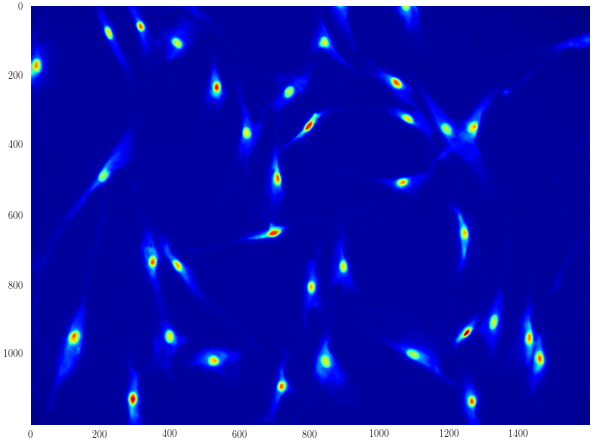
\includegraphics[scale=.64]{img/CAP3cellcorr.png}
 \caption{\small{Immagine risultante dalla correzione della disomogeneità e della fluorescenza di background sull'immagine in \figurename~\ref{fig:cell}. Si può notare (qualitativamente) come i nuclei periferici abbiano assunto un valore più simile a quelli centrali, con un maggior contrasto rispetto allo sfondo.}}
 \label{fig:cellcorr}
\end{figure}


\clearpage{\pagestyle{empty}\cleardoublepage}

\chapter{Risultati ottenuti}

\begin{flushright}\begin{small}\textit{"Hard science gives sensational results\\ with a horribly boring process."}\\
- Nassim Nicholas Taleb -\\
\end{small}\end{flushright}

Lo sviluppo e la convalida dell'algoritmo sono stati effettuati correggendo immagini in fluorescenza rossa di cellule di fibroblasti, sfruttando apposite immagini di calibrazione di sferette nanometriche, anch'esse fluorescenti nel rosso.

Le immagini di riferimento, utilizzate nella prima e nella seconda fase del programma, sono state acquisite in otto pozzetti di una multiwell: due con sferette ad intensità relativa del 100\% e due del 10\%, due con una mixture di cinque intensità (1\%, 3\%, 10\%, 30\% e 100\%) ed infine nelle rimanenti è stato posto unicamente il mezzo di coltura, così da studiare la fluorescenza di background indotta dalla sorgente.
Il riempimento di ogni pozzetto ha previsto l'agitazione sia manuale che con sonificatore delle sferette e l'iniezione con le pipette ghilson di $220\ \mu l$ di terreno completo e delle sferette di calibrazione: $10\ \mu l$ per i quattro pozzetti ad intensità unica e $2\ \mu l$ per i due pozzetti a cinque intensità.
Tuttavia una delle due immagini con sferette aventi differente luminosità ha mostrato un'errata composizione del campione e perciò è stata rimossa in fase di elaborazione e testing.

L'analisi che segue esamina l'efficacia dell'algoritmo nella rimozione della disomogeneità poiché, come visto in precedenza, il difetto della fluorescenza di sfondo viene semplicemente eliminato sottraendo il parametro costante identificato nella seconda fase.

Tale capitolo si propone di esporre e commentare i risultati conseguiti dall'algoritmo tramite due analisi: 
\begin{itemize}
 \item gli istogrammi dell'intensità dell'immagine
 \item la dipendenza dell'intensità dalla distanza dal centro
\end{itemize}

Queste due rielaborazioni verranno affrontate sulla base di grafici e risultati ottenuti applicando l'algoritmo sull'immagine dei fibroblasti, nel particolar caso in cui la prima immagine di calibrazione sia costituita da un campione di sferette con intensità relativa del 10\%.
Successivamente, per poter avere una miglior valutazione dell'efficacia del programma, verrà eseguito un confronto tra i risultati ottenuti utilizzando nella prima fase dell'algoritmo quattro distinte immagini di calibrazione, acquisite col microscopio a fluorescenza.

In Appendice B mostriamo le immagini per dare un esempio qualitativo del risultato della correzione.

\section{Distribuzione delle intensità}

Come visto, la disomogeneità di illuminazione comporta la rilevazione di immagini con intensità maggiore al centro rispetto al margine (a parità di densità di fluorocromo), comportando di conseguenza un'alterazione della distribuzione delle intensità. 
Tale fenomeno viene attenuato in modo sostanziale tramite l'azione della prima fase dell'algoritmo, la quale agisce proprio sul difetto preso in considerazione.

Il cambiamento della distribuzione di intensità provocato dal software è percepibile graficando gli istogrammi relativi alle varie intensità rilevate all'interno dell'immagine in fase pre e post correzione.
L'istogramma osservato nell'immagine non corretta è molto ampio, in quanto alla normale incertezza nel valore della fluorescenza delle sferette si aggiunge un bias legato alla loro posizione spaziale.
In seguito alla correzione ci aspettiamo un istogramma approssimativamente gaussiano con un'incertezza minore, in quanto la componente spaziale dovrebbe essere stata corretta.

In \figurename~\ref{fig:isto1} si vede l'istogramma delle intensità delle nanosfere della prima immagine di calibrazione.
È chiaramente visibile una riduzione dell'incertezza, con un picco secondario approssimativamente localizzato al doppio dell'intensità del picco primario, corrispondente alle sfere sovrapposte (dettaglio non presente nel precedente istogramma in quanto indistinguibile per via dell'ampiezza della distribuzione).
Tale risultato è proprio ciò a cui si mirava, dato che le sferette contenute nel campione risultano avere la medesima intensità.

In \figurename~\ref{fig:isto2} si vede l'istogramma logaritmico delle intensità delle nanosfere a 5 intensità. 
È chiaro il miglioramento nella qualità dell'istogramma, in cui dopo la correzione i 5 picchi sono chiaramente distinti e di ampiezza confrontabile.

In \figurename~\ref{fig:isto3} abbiamo l'istogramma dei massimi di intensità di fluorescenza delle cellule, prima e dopo la correzione.
In questo caso il miglioramento è meno visibile in quanto alle incertezze strumentali si sovrappongono quelle di natura biologica.
Per tale motivo le intensità rilevate nell'immagine è giusto che si estendano entro un range abbastanza ampio, proprio perché a seconda della concentrazione delle probes fluorescenti nella cellula sarà differente il grado di luminosità sviluppato.

\begin{figure}
 \centering
 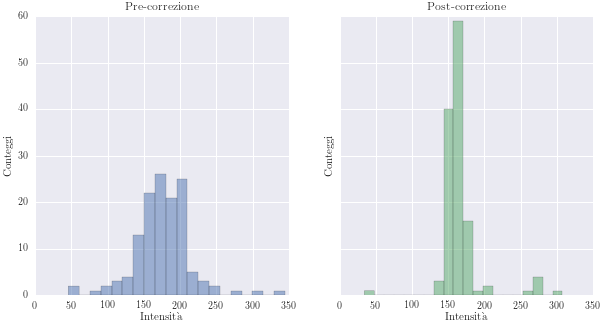
\includegraphics[scale=.55]{img/CAP4isto1.png}
 \caption{\small{Istogrammi relativi alle intensità dei massimi della prima immagine di calibrazione, costituita da sferette con stessa intensità. Il grafico a sinistra è associato alla fase di pre-correzione (\figurename~\ref{fig:unaint}), mentre quello a destra alla fase di post-correzione (\figurename~\ref{fig:unaintcorr}). Come previsto, l'algoritmo di correzione fa sì che le intensità risultino molto più piccate attorno un unico valore.}}
 \label{fig:isto1}
\end{figure}

\begin{figure}
 \centering
 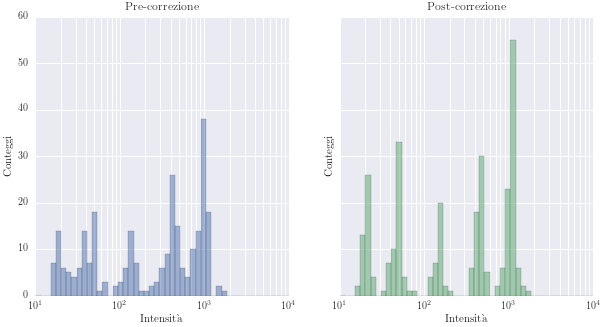
\includegraphics[scale=.55]{img/CAP4isto2.png}
 \caption{\small{Istogrammi relativi alle intensità dei massimi della seconda immagine di calibrazione, costituita da sferette con cinque intensità differenti. Il grafico a sinistra è associato alla fase di pre-correzione (\figurename~\ref{fig:piuint}), mentre quello a destra alla fase di post-correzione (\figurename~\ref{fig:piuintcorr}). Come previsto, l'algoritmo di correzione fa sì che le intensità risultino molto più piccate attorno ai cinque valori medi delle gaussiane, rendendo queste molto più definite.}}
 \label{fig:isto2}
\end{figure}

\begin{figure}
 \centering
 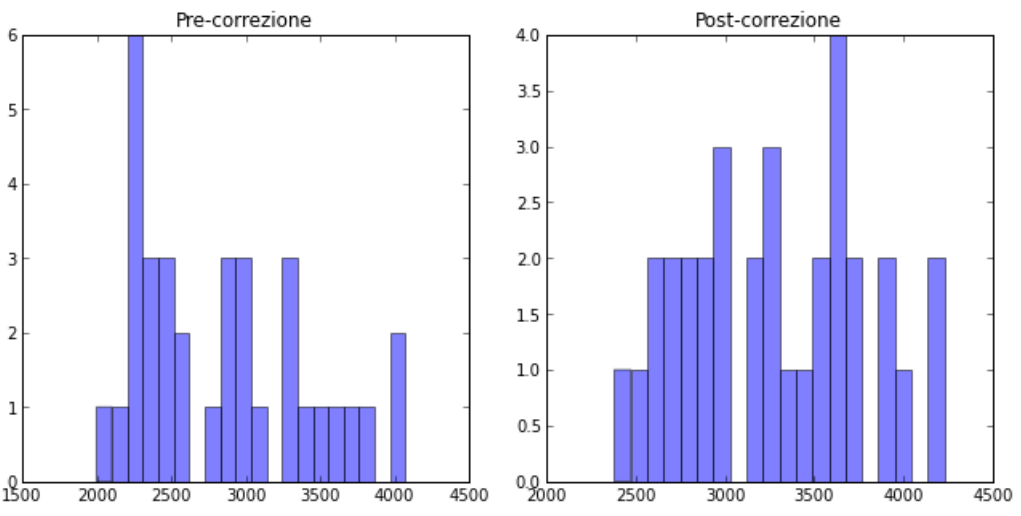
\includegraphics[scale=.55]{img/CAP4isto3.png}
 \caption{\small{Istogrammi relativi alle intensità dei massimi dell'immagine delle cellule di fibroblasti. Il grafico a sinistra è associato alla fase di pre-correzione (\figurename~\ref{fig:cell}), mentre quello a destra alla fase di post-correzione (\figurename~\ref{fig:cellcorr}). Come previsto, l'algoritmo di correzione determina una miglior simmetria della distribuzione di intensità.}}
 \label{fig:isto3}
\end{figure}


\section{Dipendenza spaziale dell'intensità}

Come criterio di evidenza della presenza o meno di una relazione fra l'intensità osservata e la posizione nel campo immagine, viene usato normalmente una soglia sul valore del p-value di questa ipotesi.
Il p-value rappresenta la plausibilità di osservare una certa relazione fra l'intensità e la posizione nel caso sia vera un'ipotesi, detta ipotesi nulla ($H_0$), secondo cui questa relazione non esista e quella osservata sia un effetto completamente casuale.
Questo criterio di selezione afferma che l'ipotesi nulla possa essere rifiutata nel caso in cui il p-value ottenuto sia inferiore ad una soglia data, normalmente assunta al valore di $0.05$.
Se la procedura di correzione funzionasse come previsto, dovremmo osservare un aumento dei p-value nei casi sotto studio.

Come precedentemente osservato, la presenza di disomogenea di illuminazione comporta una dipendenza dell'intensità dei pixel (a parità di densità di fluoroforo) dalla loro posizione.
In modo compatibile con la nostra ipotesi di lavoro stimiamo questa dipendenza come funzione della sola distanza dal centro dell'immagine.
Questa relazione non è lineare, ma è possibile calcolare il p-value di questa dipendenza approssimandolo come tale.
Il p-value rapprenta quindi la probabilità di osservare l'andamento sperimentale sotto l'ipotesi nulla che non ci sia alcuna dipendenza.

A tal proposito è stata valutata per ogni punto di massimo dell'immagine (centro delle sferette per le immagini di calibrazione e nuclei delle cellule per l'immagine da correggere) la distanza dall'origine, intesa come punto centrale dell'immagine stessa.
Le immagini sono state quindi ridotte ad una serie di coppie intensità-distanza radiale.
Per ottenere il valore del p-value si è quindi sfruttata la funzione \textit{linregress}, in grado di valutare la relazione lineare esistente o meno tra le intensità dei punti di massimo e le distanze radiali associate.
Tale funzione restituisce il p-value come semplice parametro di return e questo viene valutato prendendo come ipotesi nulla $H_0$ il fatto che la slope sia nulla, quindi minore sarà il p-value e meno plausibile sarà l'assenza di una dipendenza spaziale dell'intensità.

\begin{figure}
 \centering
 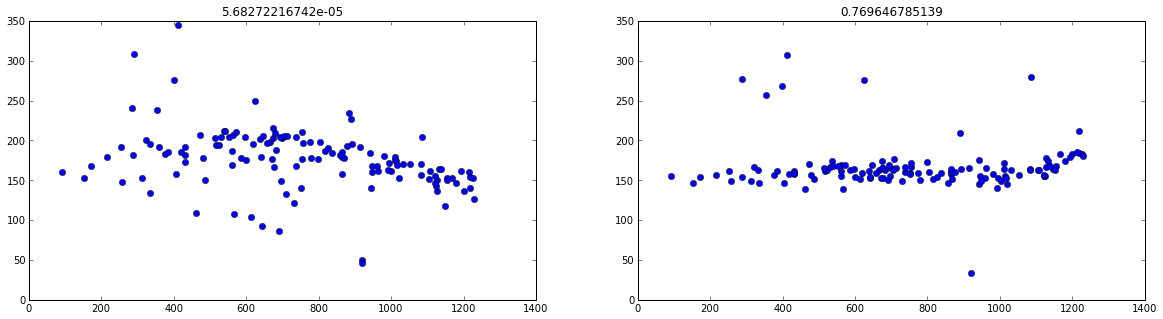
\includegraphics[scale=.55]{img/CAP4pvalue1.png}
 \caption{\small{Distribuzione delle intensità dei massimi in funzione della distanza radiale, relativa alla prima immagine di calibrazione. Il grafico in alto è associato alla fase di pre-correzione (\figurename~\ref{fig:unaint}), mentre quello in basso alla fase di post-correzione (\figurename~\ref{fig:unaintcorr}). Al di sopra sono riportati i valori del p-value associato alla corrispondente regressione lineare. Come previsto, il p-value si avvicina ad 1 una volta applicato l'algoritmo sull'immagine.}}
 \label{fig:pvalue1}
\end{figure}

\begin{figure}
 \centering
 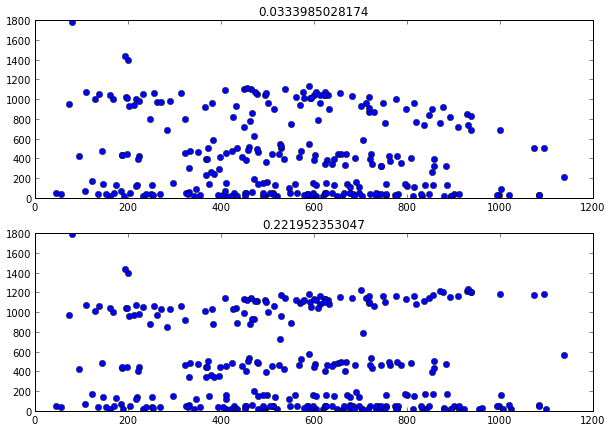
\includegraphics[scale=.55]{img/CAP4pvalue2.png}
 \caption{\small{Distribuzione delle intensità dei massimi in funzione della distanza radiale, relativa alla seconda immagine di calibrazione. Il grafico in alto è associato alla fase di pre-correzione (\figurename~\ref{fig:piuint}), mentre quello in basso alla fase di post-correzione (\figurename~\ref{fig:piuintcorr}). Al di sopra sono riportati i valori del p-value associato alla corrispondente regressione lineare. Come previsto, il p-value si avvicina ad 1 una volta applicato l'algoritmo sull'immagine.}}
 \label{fig:pvalue2}
\end{figure}

\begin{figure}
 \centering
 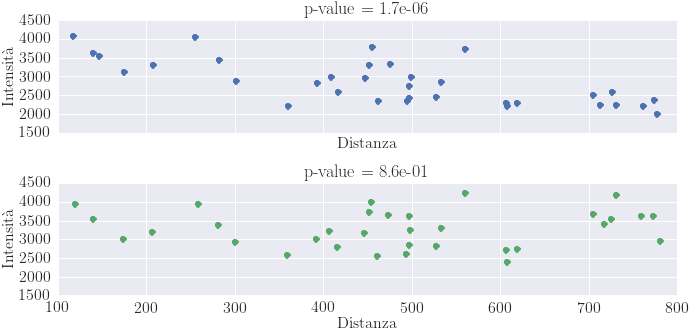
\includegraphics[scale=.55]{img/CAP4pvalue3.png}
 \caption{\small{
 Distribuzione delle intensità dei massimi in funzione della distanza radiale, relativa all'immagine delle cellule di fibroblasti. Il grafico in alto è associato alla fase di pre-correzione (\figurename~\ref{fig:cell}), mentre quello in basso alla fase di post-correzione (\figurename~\ref{fig:cellcorr}). Al di sopra sono riportati i valori del p-value associato alla corrispondente regressione lineare. Come previsto, il p-value si avvicina ad 1 una volta applicato l'algoritmo sull'immagine.}}
 \label{fig:pvalue3}
\end{figure}

Come si evince dalle Figure \ref{fig:pvalue1}, \ref{fig:pvalue2}, \ref{fig:pvalue3}, il p-value della relazione parte da valori molto bassi, che risultano significativi usando le comuni soglie di significatività.
Dopo la correzione questi risultano più elevati, compatibili con la distribuzione uniforme che ci si attende dalla distribuzione nulla.
Questo implica che dopo la correzione i dati sono compatibili con l'assenza di correlazione, sia nelle immagini di calibrazione che nell'immagine dei fibroblasti. 
Perciò, sulla base di tale analisi, dopo aver corretto l'immagine la dipendenza spaziale dell'intensità, inizialmente presente a causa della disomogeneità dell'illuminazione creata dalla sorgente, può essere considerata sostanzialmente non significativa.


\section{Confronto tra differenti immagini di calibrazione}

Come detto in precedenza, tale algoritmo permette la correzione dell'immagine a fluorescenza sulla base di due ulteriori immagini: la prima deve avere sferette di calibrazione a stessa intensità e viene sfruttata per la correzione della disomogeneità di illuminazione, mentre la seconda deve contenere sferette con differenti luminosità ed è necessaria per la rimozione del parametro di background. 
\'E sulla base di queste due ultime immagini che si ottengono i parametri necessari per la correzione di quella in esame.
Per tale motivo sono stati confrontati i risultati ottenuti con quattro distinte immagini di calibrazione ad una sola intensità: due con intensità relativa del 10\% (chiamate successivamente $10\%_1$ e $10\%_2$) e due con intensità relativa del 100\% (chiamate successivamente $100\%_1$ e $100\%_2$).

Dalle Figure \ref{fig:gauss1}, \ref{fig:gauss2}, \ref{fig:gauss3} e \ref{fig:gauss4} è evidente il fatto che differenti immagini di calibrazioni comportino differenti superfici tridimensionali risultanti dal fit di maximum likelihood, indipendentemente dall'intensità relativa delle sferette.

Per poter avere un'analisi di carattere più quantitativo sono stati visualizzati i parametri $bg,\ maxint,\ cx,\ cy,\ dsx,\ dsy,\ corr$ ed $e$ ottenuti dalla stima di massima verosimiglianza (capitolo 3.1) eseguita nei quattro casi (Figure \ref{fig:cx}, \ref{fig:cy}, \ref{fig:dsx}, \ref{fig:dsy} \ref{fig:bg}, \ref{fig:intmax}, \ref{fig:corr} e \ref{fig:e}).
Queste stime di massima verosimiglianza sono state inoltre raccolte nella \tablename~\ref{TABris}, assieme al primo parametro approssimato di background $bg_0$, calcolato inizialmente come massimo delle mode di ogni riga della matrice bidimensionale corrispondente all'immagine.

Dall'analisi di questi risultati si nota che differenti immagini di calibrazione comportano in genere differenti parametri, sebbene i valori si mantengano solitamente entro lo stesso ordine di grandezza. 
Per tale motivo si può affermare che la nostra procedura di calibrazione sembra dare una risposta coerente fra diverse immagini di calibrazione.
Tuttavia per avere una miglior valutazione dell'effetto che tali differenze potrebbero comportare sulla correzione finale dell'immagine bisognerebbe eseguire elaborazioni successive, più raffinate rispetto alla semplice analisi qui riportata.

Nelle Figure \ref{fig:c1}, \ref{fig:c2}, \ref{fig:c3}, \ref{fig:c4} sono riportate le matrici di correlazione tra le stime dei parametri per le quattro differenti immagini di calibrazione.

\begin{table}
 \begin{center}
\begin{small}
\begin{tabular}{lcccc}
\hline\hline
&$\mathbf{10\%_1}$&$\mathbf{10\%_2}$&$\mathbf{100\%_1}$&$\mathbf{100\%_2}$\\
\hline
$\mathbf{bg_0}$& 19 & 19 & 13 & 13\\
\hline
$\mathbf{cx}$&$767\pm11$&$832\pm10$&$881\pm9$&$831\pm10$\\
$\mathbf{cy}$&$587\pm9$&$583\pm7$&$583\pm6 $&$608\pm6$\\
$\mathbf{dsx}$&$823\pm205$&$ 797\pm131$&$568 \pm17$&$663\pm66$\\
$\mathbf{dsy}$&$646\pm159$&$524\pm85$&$ 409\pm11$&$453\pm44$\\
$\mathbf{corr}$&$-0.29\pm0.06$&$-0.65\pm0.05 $&$-0.51\pm0.05$&$-0.49\pm0.05$\\
$\mathbf{bg}$&$1.58\cdot 10^{-6}\pm102$&$23\pm40 $&$452\pm13$&$341\pm82$\\
$\mathbf{maxint}$&$167\pm104$&$150\pm41$&$229\pm15$&$414\pm87$\\
$\mathbf{e}$&$3.2\pm0.6$&$2.1\pm0.3$&$3.6\pm0.4$&$2.5\pm0.4$\\
\hline\hline
\end{tabular}
\caption{\small{Confronto dei parametri ottenuti nella prima fase dell'algoritmo con quattro distinte immagini di calibrazione ad una sola intensità. Per ciascun parametro del fit vengono riportate la miglior stima e la deviazione standard associata, ottenute dalla procedura di fit. La precisione dei valori risulta elevata proprio poiché non si tratta di incertezze associate alla stima, bensì dei valori che approssimano localmente la funzione di likelihood con una distribuzione gaussiana.}}
\label{TABris}
\end{small}
\end{center}
\end{table}

\clearpage

\begin{figure}
 \centering
 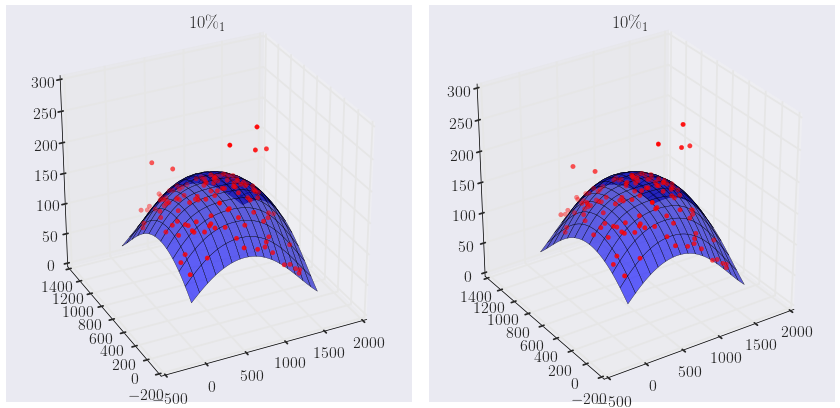
\includegraphics[scale=.45]{img/CAP4gauss1.png}
 \caption{\small{Immagine in visione ``cross eyed stereoscopic'' corrispondente alla prima immagine di calibrazione con intensità relativa del 10\%: i puntini rappresentano i massimi mentre la superficie è quella risultante dal fit di maximum likelihood.}}
 \label{fig:gauss1}
\end{figure}

\begin{figure}
 \centering
 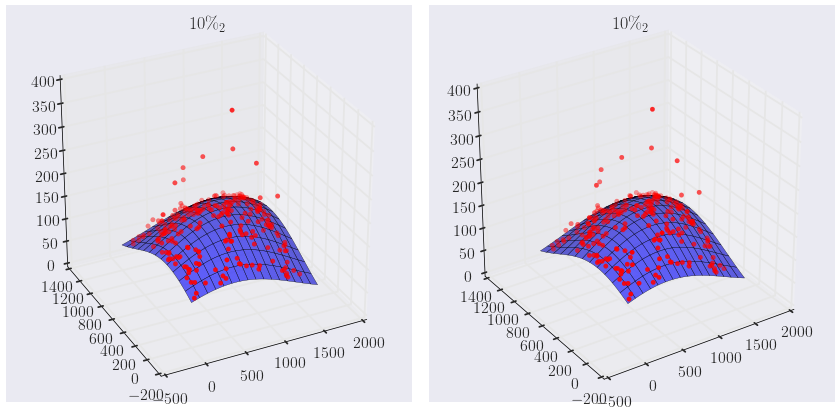
\includegraphics[scale=.45]{img/CAP4gauss2.png}
 \caption{\small{Immagine in visione ``cross eyed stereoscopic'' corrispondente alla seconda immagine di calibrazione con intensità relativa del 10\%: i puntini rappresentano i massimi mentre la superficie è quella risultante dal fit di maximum likelihood.}}
 \label{fig:gauss2}
\end{figure}

\begin{figure}
 \centering
 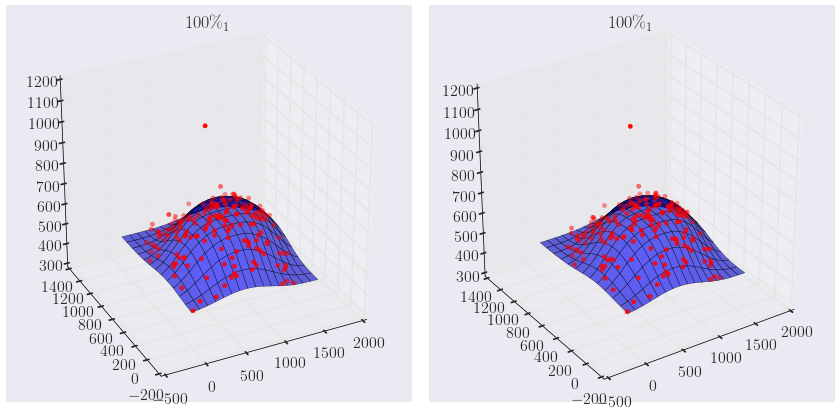
\includegraphics[scale=.45]{img/CAP4gauss3.png}
 \caption{\small{Immagine in visione ``cross eyed stereoscopic'' corrispondente alla prima immagine di calibrazione con intensità relativa del 100\%: i puntini rappresentano i massimi mentre la superficie è quella risultante dal fit di maximum likelihood.}}
 \label{fig:gauss3}
\end{figure}

\begin{figure}
 \centering
 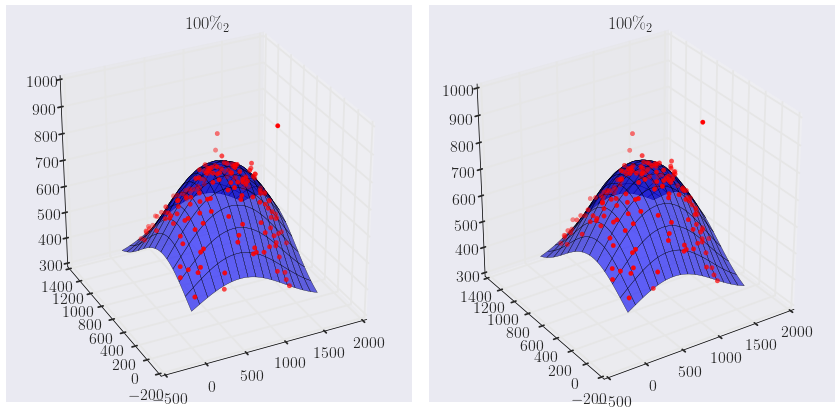
\includegraphics[scale=.45]{img/CAP4gauss4.png}
 \caption{\small{Immagine in visione ``cross eyed stereoscopic'' corrispondente alla seconda immagine di calibrazione con intensità relativa del 100\%: i puntini rappresentano i massimi mentre la superficie è quella risultante dal fit di maximum likelihood.}}
 \label{fig:gauss4}
\end{figure}


\begin{figure}
 \centering
 \includegraphics[scale=.50]{img/CAP4cx.png}
 \caption{\small{Parametro $cx$ (centro delle x) e intervallo di confidenza al 95\%, ottenuti tramite il fit di maximum likelihood presente nell'algoritmo, per le quattro differenti immagini di calibrazione ad una sola intensità.}}
 \label{fig:cx}
\end{figure}

\begin{figure}
 \centering
 \includegraphics[scale=.50]{img/CAP4cy.png}
 \caption{\small{Parametro $cy$ (centro delle y) e intervallo di confidenza al 95\%, ottenuti tramite il fit di maximum likelihood presente nell'algoritmo, per le quattro differenti immagini di calibrazione ad una sola intensità.}}
 \label{fig:cy}
\end{figure}

\begin{figure}
 \centering
 \includegraphics[scale=.50]{img/CAP4dsx.png}
 \caption{\small{Parametro $dsx$ (deviazione standard di x) e intervallo di confidenza al 95\%, ottenuti tramite il fit di maximum likelihood presente nell'algoritmo, per le quattro differenti immagini di calibrazione ad una sola intensità.}}
 \label{fig:dsx}
\end{figure}

\begin{figure}
 \centering
 \includegraphics[scale=.50]{img/CAP4dsy.png}
 \caption{\small{Parametro $dsy$ (deviazione standard di y) e intervallo di confidenza al 95\%, ottenuti tramite il fit di maximum likelihood presente nell'algoritmo, per le quattro differenti immagini di calibrazione ad una sola intensità.}}
 \label{fig:dsy}
\end{figure}

\begin{figure}
 \centering
 \includegraphics[scale=.50]{img/CAP4bg.png}
 \caption{\small{Parametro $bg$ (background) e intervallo di confidenza al 95\%, ottenuti tramite il fit di maximum likelihood presente nell'algoritmo, per le quattro differenti immagini di calibrazione ad una sola intensità.}}
 \label{fig:bg}
\end{figure}

\begin{figure}
 \centering
 \includegraphics[scale=.50]{img/CAP4intmax.png}
 \caption{\small{Parametro $maxint$ (intensità massima) e intervallo di confidenza al 95\%, ottenuti tramite il fit di maximum likelihood presente nell'algoritmo, per le quattro differenti immagini di calibrazione ad una sola intensità.}}
 \label{fig:intmax}
\end{figure}

\begin{figure}
 \centering
 \includegraphics[scale=.50]{img/CAP4corr.png}
 \caption{\small{Parametro $corr$ (correlazione tra x ed y) e intervallo di confidenza al 95\%, ottenuti tramite il fit di maximum likelihood presente nell'algoritmo, per le quattro differenti immagini di calibrazione ad una sola intensità.}}
 \label{fig:corr}
\end{figure}

\begin{figure}
 \centering
 \includegraphics[scale=.50]{img/CAP4e.png}
 \caption{\small{Parametro $e$ (esponente) e intervallo di confidenza al 95\%, ottenuti tramite il fit di maximum likelihood presente nell'algoritmo, per le quattro differenti immagini di calibrazione ad una sola intensità.}}
 \label{fig:e}
\end{figure}

\begin{figure}
 \centering
 \includegraphics[scale=.48]{img/CAP4c1.png}
 \caption{\small{Matrice di correlazione tra le stime dei parametri ottenuti dal fit di maximum likelihood per l'immagine di calibrazione $10\%_1$.}}
 \label{fig:c1}
\end{figure}

\begin{figure}
 \centering
 \includegraphics[scale=.48]{img/CAP4c2.png}
 \caption{\small{Matrice di correlazione tra le stime dei parametri ottenuti dal fit di maximum likelihood per l'immagine di calibrazione $10\%_2$.}}
 \label{fig:c2}
\end{figure}

\begin{figure}
 \centering
 \includegraphics[scale=.48]{img/CAP4c3.png}
 \caption{\small{Matrice di correlazione tra le stime dei parametri ottenuti dal fit di maximum likelihood per l'immagine di calibrazione $100\%_1$.}}
 \label{fig:c3}
\end{figure}

\begin{figure}
 \centering
 \includegraphics[scale=.48]{img/CAP4c4.png}
 \caption{\small{Matrice di correlazione tra le stime dei parametri ottenuti dal fit di maximum likelihood per l'immagine di calibrazione $100\%_2$.}}
 \label{fig:c4}
\end{figure}





\clearpage{\pagestyle{empty}\cleardoublepage}

\chapter*{Conclusioni}

\begin{flushright}
\begin{small}\textit{"Computers are useless.\\
 They can only give you answers."}\\
- Pablo Picasso -\\
\end{small}\end{flushright}

\markboth{Conclusioni}{Conclusioni}
\addcontentsline{toc}{chapter}{Conclusioni}

Obiettivo di questa tesi è la progettazione ed implementazione di un algoritmo di correzione e calibrazione di immagini generate tramite microscopia a fluorescenza.
L'algoritmo è stato calibrato usando il microscopio a fluorescenza presente nel laboratorio di biofisica del Dipartimento di Fisica ed Astronomia di Bologna.
Questa correzione ha lo scopo di migliorare l'analisi quantitativa di tali immagini, attualmente resa poco attendibile dalle varie imperfezioni ottiche presenti.
Nello specifico ci siamo proposti di correggere il difetto di non omogeneità d'illuminazione, dovuto alla forma irregolare del fascio di eccitazione, e di rimuovere la fluorescenza residua di background.

Tale correzione è basata sull'acquisizione, in parallelo al campione sotto esame, di immagini di calibrazione contenenti sfere nanometriche a fluorescenza nota.
Parte del lavoro di tesi è consistita nella generazione di diverse di queste immagini, così da poter implementare e verificare il nostro metodo di \textit{image processing}.

La correzione della luminosità è stata effettuata tramite un algoritmo da noi implementato nel linguaggio di programmazione Python.
Per la creazione di tale software di elaborazione d'immagini abbiamo ipotizzato una possibile distribuzione dell'intensità dovuta alla non omogeneità del fascio ed abbiamo quindi stimato i parametri tramite un'apposita procedura di maximum likelihood.
Per effettuare questa stima abbiamo anche tenuto conto di possibili effetti dovuti alla luminosità di background, alla sovrapposizione di più nanosfere e ad effetti di bordo nel corso dell'elaborazione.
Questa procedura è stata ripetuta su quattro diverse immagini di calibrazione, per valutarne la consistenza e l'efficacia.

Per verificare che la procedura ideata abbia le desiderate proprietà di linearità fra segnale misurato ed intensità nota, ci siamo serviti di un'ulteriore immagine di calibrazione contenente una mistura di sfere nanometriche con intensità variabili su due ordini di grandezza.
Grazie ad essa abbiamo verificato che la nostra procedura incrementa la discriminazione tra queste intensità e che il segnale risultante può essere facilmente mappato su una scala lineare. 

Dall'analisi dei risultati ottenuti, la nostra procedura di calibrazione sembra dare una risposta coerente fra diverse immagini di calibrazione ed un segnale compatibile con le proprietà desiderate di linearità e di indipendenza dalla posizione all'interno dell'immagine. 
Questo algoritmo verrà quindi inserito in un programma che permetterà la calibrazione delle immagini in microscopia a fluorescenza nei futuri esperimenti del laboratorio di biofisica.

Per un futuro completamente della calibrazione del microscopio, successivamente a questo lavoro i tesi, sarà necessario includere addizionali metodi di correzione per tener conto di altre fonti di incertezza.
Per prima cosa bisognerà ripetere l'acquisizione di immagini di calibrazione su più esperimenti, così da decidere se sia necessaria una calibrazione individuale per ciascun esperimento o se sia possibile una calibrazione generale, indipendentemente dal singolo esperimento.
Dovranno essere valutati anche gli effetti di distorsione legati al sistema ottico, come aberrazioni sferiche, coma, astigmatismo e distorsione.
Sarà poi importante valutare l'allineamento fra le immagini acquisite in campo chiaro e con diversi tipi di fluorescenza e stimare la Point Spread Function (PSF) del microscopio su ciascuna frequenza, per poter effettuare una deconvoluzione dell'immagine in grado di ridurre la perdita di risoluzione dovuta alla diffrazione.



\appendix
\clearpage{\pagestyle{empty}\cleardoublepage}
\chapter{Codice Sorgente} 
\label{appendiceWSS} 

\lstset{language=Python, numbers=left, stepnumber=1, breaklines=true}

\begin{lstlisting}
from __future__ import division
import pylab
from pylab import *
from scipy.optimize import curve_fit
import numpy as np
import scipy
import scipy.ndimage as ndimage
import scipy.ndimage.filters as filters
import matplotlib.pyplot as plt
import itertools
import scipy.stats as st
from mpl_toolkits.mplot3d import Axes3D
from scipy.stats.mstats import mquantiles
import numexpr as ne
import PyZenity
from scipy.ndimage.filters import gaussian_filter
from sklearn import mixture
import matplotlib
matplotlib.rc('font',**{'family':'serif','serif':['Computer Modern']})
matplotlib.rc('text', usetex=True)
import seaborn as sbn
from matplotlib import rcParams
rcParams["text.latex.unicode"]=True
rcParams["font.size"]=16
rcParams["axes.titlesize"]=18
rcParams["axes.labelsize"]=16
rcParams["xtick.labelsize"]=16
rcParams["ytick.labelsize"]=16
rcParams["figure.dpi"]=80
from matplotlib.colorbar import make_axes


# DEFINIZIONE DELLE FUNZIONI ----------
# Calcolo dell'intensita (integrale media) associata ad un massimo 
def intensity(x, y, imm):
    z = []    
    delta = 5
    for xi, yi in zip(x, y):
        val = 0
        count = 0
        for i in range(-delta, delta):
            for j in range(-delta, delta):
                if imm[yi+i,xi+j]>0:
                    count=count+1
                    val = val + imm[yi+i, xi+j]
        z.append(val/count)  
    z = np.array(z)
    return z
        
# Funzione di ricerca dei massimi 
def find_max(imm):
    vicinanza_size = 10
    imm_max = filters.maximum_filter(imm, vicinanza_size)
    maxima = (imm == imm_max)
    imm_min = filters.minimum_filter(imm, vicinanza_size)
    soglia = 40
    diff = ((imm_max - imm_min) > soglia)
    maxima[diff == 0] = 0
    labeled, num_objects = ndimage.label(maxima)
    slices = ndimage.find_objects(labeled)
    margine = 50
    x, y = [], []
    for dy,dx in slices:
        x_center = (dx.start + dx.stop - 1)//2
        y_center = (dy.start + dy.stop - 1)//2 
        if x_center<margine or x_center>imm.shape[1]-margine:
            continue                                         
        if y_center<margine or y_center>imm.shape[0]-margine:
            continue
        x.append(x_center)
        y.append(y_center)
    x = np.array(x)
    y = np.array(y)
    z = intensity(x, y, imm)
    return x, y, z

# Ricerca della funzione ''gauss'' che fitta al meglio i massimi
def gauss(x, y, dsx, dsy, maxint, corr, cx, cy, bg, e):
        if dsx<0:
            return np.nan
        if dsy<0:
            return np.nan
        if maxint<0:
            return np.nan
        if cx<0:
            return np.nan
        if cy<0:
            return np.nan
        if bg<0: 
            return np.nan
        if ((corr<-1) or (corr>1)):
            return np.nan
        if e<0:
            return np.nan
        varx =((x-cx)/dsx)**2
        vary = ((y-cy)/dsy)**2
        varxy = (corr*(x-cx)*(y-cy))/(dsy*dsx)
        d = sqrt(varx+vary+varxy)
        return ne.evaluate('bg + maxint * exp( -0.5 * d**e )')
        
# Ricerca dei parametri della curva ''gauss''
def analyze(imm):
    x, y, z = find_max(imm)
    xy = array(zip(x, y))
    def gauss_for_curve(xy, *args):
        x, y = xy.T
        return gauss(x, y, *args)
    parametri_0 = (800, 600, np.max(imm), 0, 800, 600, 0, 2)
    parametri, covar = curve_fit(gauss_for_curve, xy, z, parametri_0)
    imm_normalized = correction(imm, parametri)
    # Esclusione dei punti più intensi
    quantile = mquantiles(imm_normalized[y, x], 0.95)
    newx, newy = [], []
    for (valore, xtemp, ytemp) in zip(imm_normalized[y, x], x, y):
        if valore < quantile:
            newy.append(ytemp) 
            newx.append(xtemp)
    newx = asarray(newx) 
    newy = asarray(newy)
    newz = intensity(newx, newy, imm)
    newxy = array(zip(newx, newy))
    newparametri, newcovar = curve_fit(gauss_for_curve, newxy, newz, parametri)
    print newparametri
    return newparametri

# Correzione dell'immagine sulla base dei parametri della curva ''gauss''
def correction(imm, par):

    xx, yy = np.meshgrid(np.linspace(0, 1600, 1600), np.linspace(0, 1200, 1200))
    
    zz = gauss(xx, yy, *par)
    
    zz_normalized = zz / np.max(zz)
    imm_normalized = imm/zz_normalized
    return imm_normalized 
# -------------------------------------


# Fase I: EFFETTO DEI BORDI - IMMAGINE DELLE SFERETTE AD UNA SOLA INTENSITA
# Inserimento immagine da utente
fname_sfere = PyZenity.GetFilename()[0]
imm = pylab.imread(fname_sfere)
# Applicazione filtro gaussiano
imm = gaussian_filter(imm, 2)
# Sottrazione della prima approssimazione del background
mode = max(scipy.stats.mode(imm)[0][0])
imm = imm - mode
# Ricerca dei parametri della curva ''gauss''
par = analyze(imm)
# Autocorrezione dell'immagine delle sferette ad una sola intensita
corretta = correction(imm, par)
######x, y, z = find_max(corretta)


# Fase II: LINEARITA - IMMAGINE DELLE SFERETTE CON MIX DI INTENSITA
# Inserimento immagine da utente
fname_sferemix = PyZenity.GetFilename()[0]
imm1 = pylab.imread(fname_sferemix)
# Applicazione filtro gaussiano e sottrazione della prima approssimazione del background
imm1 = gaussian_filter(imm1, 2)
imm1 = imm1 - mode
# Correzione dell'immagine delle sferette con mix di intensita
corretta1 = correction(imm1, par)
# Identificazione dei centri delle sferette, ossia dei massimi
x1, y1, z1 = find_max(corretta1)
# Studio della risposta lineare con il gaussian mixture
clf = mixture.GMM(n_components = 5, n_init = 100, init_params = '', params = 'mwc') 
clf.weights_ = asarray([0.2]*5)
clf.means_ = asarray((3.0, 4.0, 5.0, 6.0, 7.0)).reshape(5, 1)
clf.covars_ = asarray([0.015]*5).reshape(5,1)
clf.fit(log(z1))
intnote = log([1, 3, 10, 33, 100])
parlin = st.linregress(exp(intnote), exp(clf.means_.ravel()))
def linreg(x, A, B):
    return A*x+B
x = exp(intnote)
y = exp(clf.means_.ravel())
erry = exp(clf.covars_.ravel())
param0 = [parlin[0], parlin[1]]
param, varpar = curve_fit(linreg, x, y, p0 = param0, sigma = erry)
errpar = (diag(varpar))**(1/2)
corretta1 = corretta1 - param[1]


# CORREZIONE DELL'IMMAGINE DI CELLULE A FLUORESCENZA
# Inserimento immagine da utente
cell = PyZenity.GetFilename()[0]
imm_cell_0 = pylab.imread(cell)
# Applicazione filtro gaussiano e sottrazione della prima approssimazione del background
imm_cell = gaussian_filter(imm_cell_0, 2)
imm_cell = imm_cell - mode
# Risposta lineare: sottrazione del parametro di background rivelato dalla fase II
imm_cell_corr = imm_cell - param[1]
# Effetto dei bordi: correzione tramite i parametri calcolati nella fase I
imm_cell_corr = correction(imm_cell_corr, par)
# Salvataggio dell'immagine delle cellule corretta
scipy.misc.imsave('Corretta.tif', imm_cell_corr)
\end{lstlisting}


%\addtolength{\parskip}{5pt}


\clearpage{\pagestyle{empty}\cleardoublepage}

\begin{thebibliography}{3}

\addcontentsline{toc}{chapter}{Bibliografia}


\bibitem{storia} Marco Brusadin (2010), \emph{"La microscopia in fluorescenza"} \newline  http://www.marcobrusadin.it

\bibitem{fluo} Waters, J.C., and Swedlow, J.R. (2007), \emph {"Interpreting Fluorescence Microscopy Images and Measurements. In Evaluating Techniques in Biochemical Research"} \newline D. Zuk, ed. (Cambridge, MA: Cell Press), \newline http://www.cellpress.com/misc/page?page=ETBR.

\bibitem{quantumyield} A. M. Brouwer \emph{"Standards for photoluminescence quantum yield measurements in solution (IUPAC Technical Report)"} \newline Pure Appl. Chem., 2011, Vol. 83, No. 12, pp. 2213-2228

\bibitem{quenching} F.W.D. Rost (1996), \emph{"Fluorescence microscopy"} \newline ed. Cambridge University Press

\bibitem{concquenc} David Peak (1983), \emph{"Fluorescence quenching at high quencher concentrations"} \newline J. Chem. Phys. 79, 3328, doi:10.1063/1.446234

\bibitem{tecniche} J.B. Pawley (2006), \emph{"Handbook of biological confocal microscopy"} \newline ed. Springer

\bibitem{NA} M.E. Dailey, A. Khodjakov, C.L. Rieder, M. Platani, J.R. Swedlow, P.D. Andrews, Yu-li Wang, J.C. Waters, N.S. Claxton, S.G. Olenych, J.D. Griffin and M.W. Davidson, \emph{"Optical system and detector requirements for live-cell imaging"} \newline http://www.microscopyu.com/articles/livecellimaging/imagingsystems.html

\bibitem{Nikon1} M.W. Davidson, K.R. Spring (2006), \emph{"Introduction to fluorescence microscopy - Nikon microscopy, the source for microscopy education"} \newline [Online; accessed 15-October-2010, Nikon]

\bibitem{Nikon2} S.A. Schwartz, M.W. Davidson, J.S. Silfies, E.G. Lieser (2010), \emph{"Nikon perfect focus system - Nikon microscopy, the source for microscopy education"} \newline [Online; accessed 19-October-2010, Nikon]

\bibitem{difetti} G. Pietro Sini, Donato Di Ferdinando, Gabriele Sirri (2013), \emph{"Problemi tecnici della microscopia ottica"} \newline http://www.funsci.com/fun3\_it/sini/mo/m\_ottica.htm

\bibitem{nigro} P. Mazzoldi, M. Nigro, C. Voci (2007), \emph{"Fisica - Volume II"} \newline ed. EdiSES

\bibitem{decon} Dr. David S.C. Biggs (2004), \emph{"Biophotonics International, photonic solutions for biotechnology and medicine - Clearing Up Deconvolution"} \newline ed. Laurin Publishing Co. Inc.

\bibitem{python} A. Downey, J. Elkner, C. Meyers (2002), \emph{"How to Think Like a Computer Scientist - Learning with Python"} \newline Green Tea Press, Wellesley (Massachusetts)

\end{thebibliography} 


\clearpage{\pagestyle{empty}\cleardoublepage}
\chapter*{Rigraziamenti}
\fancyhf{} %Clears all header and footer fields, in preparation.
\addtolength{\parskip}{- 5pt}

Qui ringrazio tutti!


\end{document}